\UseRawInputEncoding
%DIF LATEXDIFF DIFFERENCE FILE
%DIF DEL ./old/compiled_vXXX_submitted_base.tex   Fri May 24 09:29:57 2024
%DIF ADD ./compiled.tex                           Sun May 26 15:11:02 2024

%%%%%%%%%%%%%%%%%%%%%%%%%%%%%%%%%%%%%%%%%%%%%%%%%%%%%%%%%%%%%%%%%%%%%%%%%%%%%%%%
%% SETTINGS
%%%%%%%%%%%%%%%%%%%%%%%%%%%%%%%%%%%%%%%%%%%%%%%%%%%%%%%%%%%%%%%%%%%%%%%%%%%%%%%%
%% Columns
%DIF 7c7
%DIF < \documentclass[final,3p,times,twocolumn]{elsarticle}
%DIF -------
%% \documentclass[final,3p,times,twocolumn]{elsarticle} %% Use it for submission %DIF > 
%DIF -------
%% Use the options 1p,twocolumn; 3p; 3p,twocolumn; 5p; or 5p,twocolumn
%% for a journal layout:
%% \documentclass[final,1p,times]{elsarticle}
%% \documentclass[final,1p,times,twocolumn]{elsarticle}
%% \documentclass[final,3p,times]{elsarticle}
%% \documentclass[final,3p,times,twocolumn]{elsarticle}
%% \documentclass[final,5p,times]{elsarticle}
%% \documentclass[final,5p,times,twocolumn]{elsarticle}
%DIF 16c16
%DIF < %% \documentclass[preprint,review,12pt]{elsarticle}%% preamble
%DIF -------
\documentclass[preprint,review,12pt]{elsarticle}%% preamble %DIF > 
%DIF -------
\usepackage[english]{babel}
\usepackage[table]{xcolor} % For coloring tables
\usepackage{booktabs} % For professional quality tables
\usepackage{colortbl} % For coloring cells in tables
\usepackage{amsmath, amssymb} % For mathematical symbols and environments
\usepackage{amsthm} % For theorem-like environments
\usepackage{lipsum} % just for sample text
\usepackage{natbib}
\usepackage{graphicx}
\usepackage{indentfirst}
\usepackage{bashful}
\usepackage[margin=10pt,font=small,labelfont=bf,labelsep=endash]{caption}
\usepackage{graphicx}
\usepackage{calc}
\usepackage[T1]{fontenc} % [REVISED]
\usepackage[utf8]{inputenc} % [REVISED]
\usepackage{hyperref}
\usepackage{accsupp}
% Tables
\usepackage[pass]{geometry}
\usepackage{pdflscape}
\usepackage{csvsimple}
\usepackage{xltabular}
\usepackage{booktabs}
\usepackage{siunitx}
\usepackage{makecell}
\sisetup{round-mode=figures,round-precision=3}
\renewcommand\theadfont{\bfseries}
\renewcommand\theadalign{c}
\newcolumntype{C}[1]{>{\centering\arraybackslash}m{#1}}
\renewcommand{\arraystretch}{1.5}
\definecolor{lightgray}{gray}{0.95}

%% Diff
\usepackage{xcolor}
\usepackage[most]{tcolorbox} % for boxes with transparency

%% Image width
\newlength{\imagewidth}
\newlength{\imagescale}

%% Line numbers
\linespread{1.2}
\linenumbers

% Define colors with transparency (opacity value)
\definecolor{GreenBG}{rgb}{0,1,0}
\definecolor{RedBG}{rgb}{1,0,0}
% Define tcolorbox environments for highlighting
\newtcbox{\greenhighlight}[1][]{%
  on line,
  colframe=GreenBG,
  colback=GreenBG!50!white, % 50% transparent green
  boxrule=0pt,
  arc=0pt,
  boxsep=0pt,
  left=1pt,
  right=1pt,
  top=2pt,
  bottom=2pt,
  tcbox raise base
}
\newtcbox{\redhighlight}[1][]{%
  on line,
  colframe=RedBG,
  colback=RedBG!50!white, % 50% transparent red
  boxrule=0pt,
  arc=0pt,
  boxsep=0pt,
  left=1pt,
  right=1pt,
  top=2pt,
  bottom=2pt,
  tcbox raise base
}
\newcommand{\REDSTARTS}{\color{red}}
\newcommand{\REDENDS}{\color{black}}
\newcommand{\GREENSTARTS}{\color{green}}
\newcommand{\GREENENDS}{\color{black}}

% New command to read word counts
\newread\wordcount
\newcommand\readwordcount[1]{%
  \openin\wordcount=#1
  \read\wordcount to \thewordcount
  \closein\wordcount
  \thewordcount
}


%%%%%%%%%%%%%%%%%%%%%%%%%%%%%%%%%%%%%%%%%%%%%%%%%%%%%%%%%%%%%%%%%%%%%%%%%%%%%%%%
%% JOURNAL NAME
%%%%%%%%%%%%%%%%%%%%%%%%%%%%%%%%%%%%%%%%%%%%%%%%%%%%%%%%%%%%%%%%%%%%%%%%%%%%%%%%
\journal{Heliyon}
%%%%%%%%%%%%%%%%%%%%%%%%%%%%%%%%%%%%%%%%%%%%%%%%%%%%%%%%%%%%%%%%%%%%%%%%%%%%%%%%
%% DOCUMENT STARTS
%%%%%%%%%%%%%%%%%%%%%%%%%%%%%%%%%%%%%%%%%%%%%%%%%%%%%%%%%%%%%%%%%%%%%%%%%%%%%%%%
%DIF PREAMBLE EXTENSION ADDED BY LATEXDIFF
%DIF UNDERLINE PREAMBLE %DIF PREAMBLE
\RequirePackage[normalem]{ulem} %DIF PREAMBLE
\RequirePackage{color}\definecolor{RED}{rgb}{1,0,0}\definecolor{BLUE}{rgb}{0,0,1} %DIF PREAMBLE
\providecommand{\DIFaddtex}[1]{{\protect\color{blue}\uwave{#1}}} %DIF PREAMBLE
\providecommand{\DIFdeltex}[1]{{\protect\color{red}\sout{#1}}}                      %DIF PREAMBLE
%DIF SAFE PREAMBLE %DIF PREAMBLE
\providecommand{\DIFaddbegin}{} %DIF PREAMBLE
\providecommand{\DIFaddend}{} %DIF PREAMBLE
\providecommand{\DIFdelbegin}{} %DIF PREAMBLE
\providecommand{\DIFdelend}{} %DIF PREAMBLE
\providecommand{\DIFmodbegin}{} %DIF PREAMBLE
\providecommand{\DIFmodend}{} %DIF PREAMBLE
%DIF FLOATSAFE PREAMBLE %DIF PREAMBLE
\providecommand{\DIFaddFL}[1]{\DIFadd{#1}} %DIF PREAMBLE
\providecommand{\DIFdelFL}[1]{\DIFdel{#1}} %DIF PREAMBLE
\providecommand{\DIFaddbeginFL}{} %DIF PREAMBLE
\providecommand{\DIFaddendFL}{} %DIF PREAMBLE
\providecommand{\DIFdelbeginFL}{} %DIF PREAMBLE
\providecommand{\DIFdelendFL}{} %DIF PREAMBLE
%DIF HYPERREF PREAMBLE %DIF PREAMBLE
\providecommand{\DIFadd}[1]{\texorpdfstring{\DIFaddtex{#1}}{#1}} %DIF PREAMBLE
\providecommand{\DIFdel}[1]{\texorpdfstring{\DIFdeltex{#1}}{}} %DIF PREAMBLE
\newcommand{\DIFscaledelfig}{0.5}
%DIF HIGHLIGHTGRAPHICS PREAMBLE %DIF PREAMBLE
\RequirePackage{settobox} %DIF PREAMBLE
\RequirePackage{letltxmacro} %DIF PREAMBLE
\newsavebox{\DIFdelgraphicsbox} %DIF PREAMBLE
\newlength{\DIFdelgraphicswidth} %DIF PREAMBLE
\newlength{\DIFdelgraphicsheight} %DIF PREAMBLE
% store original definition of \includegraphics %DIF PREAMBLE
\LetLtxMacro{\DIFOincludegraphics}{\includegraphics} %DIF PREAMBLE
\newcommand{\DIFaddincludegraphics}[2][]{{\color{blue}\fbox{\DIFOincludegraphics[#1]{#2}}}} %DIF PREAMBLE
\newcommand{\DIFdelincludegraphics}[2][]{% %DIF PREAMBLE
\sbox{\DIFdelgraphicsbox}{\DIFOincludegraphics[#1]{#2}}% %DIF PREAMBLE
\settoboxwidth{\DIFdelgraphicswidth}{\DIFdelgraphicsbox} %DIF PREAMBLE
\settoboxtotalheight{\DIFdelgraphicsheight}{\DIFdelgraphicsbox} %DIF PREAMBLE
\scalebox{\DIFscaledelfig}{% %DIF PREAMBLE
\parbox[b]{\DIFdelgraphicswidth}{\usebox{\DIFdelgraphicsbox}\\[-\baselineskip] \rule{\DIFdelgraphicswidth}{0em}}\llap{\resizebox{\DIFdelgraphicswidth}{\DIFdelgraphicsheight}{% %DIF PREAMBLE
\setlength{\unitlength}{\DIFdelgraphicswidth}% %DIF PREAMBLE
\begin{picture}(1,1)% %DIF PREAMBLE
\thicklines\linethickness{2pt} %DIF PREAMBLE
{\color[rgb]{1,0,0}\put(0,0){\framebox(1,1){}}}% %DIF PREAMBLE
{\color[rgb]{1,0,0}\put(0,0){\line( 1,1){1}}}% %DIF PREAMBLE
{\color[rgb]{1,0,0}\put(0,1){\line(1,-1){1}}}% %DIF PREAMBLE
\end{picture}% %DIF PREAMBLE
}\hspace*{3pt}}} %DIF PREAMBLE
} %DIF PREAMBLE
\LetLtxMacro{\DIFOaddbegin}{\DIFaddbegin} %DIF PREAMBLE
\LetLtxMacro{\DIFOaddend}{\DIFaddend} %DIF PREAMBLE
\LetLtxMacro{\DIFOdelbegin}{\DIFdelbegin} %DIF PREAMBLE
\LetLtxMacro{\DIFOdelend}{\DIFdelend} %DIF PREAMBLE
\DeclareRobustCommand{\DIFaddbegin}{\DIFOaddbegin \let\includegraphics\DIFaddincludegraphics} %DIF PREAMBLE
\DeclareRobustCommand{\DIFaddend}{\DIFOaddend \let\includegraphics\DIFOincludegraphics} %DIF PREAMBLE
\DeclareRobustCommand{\DIFdelbegin}{\DIFOdelbegin \let\includegraphics\DIFdelincludegraphics} %DIF PREAMBLE
\DeclareRobustCommand{\DIFdelend}{\DIFOaddend \let\includegraphics\DIFOincludegraphics} %DIF PREAMBLE
\LetLtxMacro{\DIFOaddbeginFL}{\DIFaddbeginFL} %DIF PREAMBLE
\LetLtxMacro{\DIFOaddendFL}{\DIFaddendFL} %DIF PREAMBLE
\LetLtxMacro{\DIFOdelbeginFL}{\DIFdelbeginFL} %DIF PREAMBLE
\LetLtxMacro{\DIFOdelendFL}{\DIFdelendFL} %DIF PREAMBLE
\DeclareRobustCommand{\DIFaddbeginFL}{\DIFOaddbeginFL \let\includegraphics\DIFaddincludegraphics} %DIF PREAMBLE
\DeclareRobustCommand{\DIFaddendFL}{\DIFOaddendFL \let\includegraphics\DIFOincludegraphics} %DIF PREAMBLE
\DeclareRobustCommand{\DIFdelbeginFL}{\DIFOdelbeginFL \let\includegraphics\DIFdelincludegraphics} %DIF PREAMBLE
\DeclareRobustCommand{\DIFdelendFL}{\DIFOaddendFL \let\includegraphics\DIFOincludegraphics} %DIF PREAMBLE
%DIF LISTINGS PREAMBLE %DIF PREAMBLE
\RequirePackage{listings} %DIF PREAMBLE
\RequirePackage{color} %DIF PREAMBLE
\lstdefinelanguage{DIFcode}{ %DIF PREAMBLE
%DIF DIFCODE_UNDERLINE %DIF PREAMBLE
  moredelim=[il][\color{red}\sout]{\%DIF\ <\ }, %DIF PREAMBLE
  moredelim=[il][\color{blue}\uwave]{\%DIF\ >\ } %DIF PREAMBLE
} %DIF PREAMBLE
\lstdefinestyle{DIFverbatimstyle}{ %DIF PREAMBLE
	language=DIFcode, %DIF PREAMBLE
	basicstyle=\ttfamily, %DIF PREAMBLE
	columns=fullflexible, %DIF PREAMBLE
	keepspaces=true %DIF PREAMBLE
} %DIF PREAMBLE
\lstnewenvironment{DIFverbatim}{\lstset{style=DIFverbatimstyle}}{} %DIF PREAMBLE
\lstnewenvironment{DIFverbatim*}{\lstset{style=DIFverbatimstyle,showspaces=true}}{} %DIF PREAMBLE
%DIF END PREAMBLE EXTENSION ADDED BY LATEXDIFF

\begin{document}

%%%%%%%%%%%%%%%%%%%%%%%%%%%%%%%%%%%%%%%%%%%%%%%%%%%%%%%%%%%%%%%%%%%%%%%%%%%%%%%%
%% Frontmatter
%%%%%%%%%%%%%%%%%%%%%%%%%%%%%%%%%%%%%%%%%%%%%%%%%%%%%%%%%%%%%%%%%%%%%%%%%%%%%%%%
\begin{frontmatter}
\begin{highlights}
\pdfbookmark[1]{Highlights}{highlights}

\item Neural trajectories in the hippocampus exhibited greater variability during a working memory (WM) task compared to those in the entorhinal cortex and amygdala regions.

\item The distance of neural trajectories between encoding and retrieval states in the hippocampus was memory-load dependent during a WM task.


\item Hippocampal neural trajectories fluctuated between the encoding and retrieval states in a task-dependent manner during both baseline and sharp-wave ripple (SWR) periods.

\item Hippocampal neural trajectories shifted from encoding to retrieval states during SWR period.

\end{highlights}\title{
Hippocampal Neural Fluctuations Between Memory Encoding and Retrieval States During a Working Memory Task in Humans
}\author[1]{Yusuke Watanabe\corref{cor1}}
\author[2,3,4]{Yuji Ikegaya}
\author[1,5]{Takufumi Yanagisawa}

\address[1]{Institute for Advanced Cocreation studies, Osaka University, 2-2 Yamadaoka, Suita, 565-0871, Osaka, Japan}
\address[2]{Graduate School of Pharmaceutical Sciences, The University of Tokyo, 7-3-1 Hongo, Tokyo, 113-0033, Japan}
\address[3]{Institute for AI and Beyond, The University of Tokyo, 7-3-1 Hongo, Tokyo, 113-0033, Japan}
\address[4]{Center for Information and Neural Networks, National Institute of Information and Communications Technology, 1-4 Yamadaoka, Suita City, 565-0871, Osaka, Japan}
\address[5]{Department of Neurosurgery, Osaka University Graduate School of Medicine, 2-2 Yamadaoka, Osaka, 565-0871, Japan}

\cortext[cor1]{Corresponding author. Tel: +81-6-6879-3652 Email: ywatanabe@alumni.u-tokyo.ac.jp}

%%Graphical abstract
%\pdfbookmark[1]{Graphical Abstract}{graphicalabstract}        
%\begin{graphicalabstract}
%\includegraphics{grabs}
%\end{graphicalabstract}
\begin{abstract}
  \pdfbookmark[1]{Abstract}{abstract}
Working memory (WM) is crucial for a multitude of cognitive functions, but its underlying neural mechanisms at play remain to be fully understood. Interestingly, the hippocampus and sharp-wave ripples (SWRs)--- transient and synchronous oscillation observed in the hippocampus --- garner recognition for their significance in memory consolidation and retrieval, albeit their correlation with WM tasks remains to be elucidated. Here we show that during a WM task, multi-unit activity patterns in the hippocampus display distinctive dynamics, especially during SWR periods. This study analyzed intracranial electroencephalography data from the medial temporal lobe (MTL) of nine patients with epilepsy, recorded during an eight-second Sternberg task. Utilizing Gaussian-process factor analysis, we extracted low-dimensional neural representations or trajectories (NT) within MTL regions during the Sternberg WM task. The results revealed significant variations in NT of the hippocampus compared to those of the entorhinal cortex and the amygdala. Additionally, the distance of the NT between the encoding and retrieval phases was dependent on memory load. Crucially, hippocampal NT oscillated during the retrieval phase between encoding and retrieval states in a task-dependent manner. Notably, these fluctuations shifted from encoding to retrieval states during SWR episodes. These findings reaffirm the role of the hippocampus in WM tasks and propose a hypothesis: the hippocampus transitions its functional state from encoding to retrieval during SWRs in WM tasks.
\end{abstract}

% \pdfbookmark[1]{Keywords}{keywords}                
\begin{keyword}
working memory \sep memory load \sep hippocampus \sep sharp-wave ripples \sep humans
\end{keyword}
\end{frontmatter}

%%%%%%%%%%%%%%%%%%%%%%%%%%%%%%%%%%%%%%%%%%%%%%%%%%%%%%%%%%%%%%%%%%%%%%%%%%%%%%%%
%% Counters
%%%%%%%%%%%%%%%%%%%%%%%%%%%%%%%%%%%%%%%%%%%%%%%%%%%%%%%%%%%%%%%%%%%%%%%%%%%%%%%%
\DIFdelbegin %DIFDELCMD < \begin{wordcount*}
%DIFDELCMD < %%%
\DIFdelend \DIFaddbegin \begin{*wordcount}
\DIFaddend \readwordcount{./src/.figure_count.txt} figures, \readwordcount{./src/.table_count.txt} tables, \readwordcount{./src/.abstract_count.txt} words for abstract, and \readwordcount{./src/.imrd_count.txt} words for main text
\DIFdelbegin %DIFDELCMD < \end{wordcount*}
%DIFDELCMD < %%%
\DIFdelend \DIFaddbegin \end{*wordcount}
\DIFaddend %%%%%%%%%%%%%%%%%%%%%%%%%%%%%%%%%%%%%%%%%%%%%%%%%%%%%%%%%%%%%%%%%%%%%%%%%%%%%%%%
%% IMRaD
%%%%%%%%%%%%%%%%%%%%%%%%%%%%%%%%%%%%%%%%%%%%%%%%%%%%%%%%%%%%%%%%%%%%%%%%%%%%%%%%

%%%%%%%%%%%%%%%%%%%%%%%%%%%%%%%%%%%%%%%%%%%%%%%%%%%%%%%%%%%%%%%%%%%%%%%%%%%%%%%%
%% INTRODUCTION
%%%%%%%%%%%%%%%%%%%%%%%%%%%%%%%%%%%%%%%%%%%%%%%%%%%%%%%%%%%%%%%%%%%%%%%%%%%%%%%%
\section{Introduction}
Working memory (WM)\DIFdelbegin \DIFdel{is crucial in everyday life; however, its neural mechanism has yet to be fully elucidated. Specifically, the hippocampus's involvement in WM processing, a pivotal region for memory, is the subject of ongoing research \mbox{%DIFAUXCMD
\cite{scoville_loss_1957} }\hspace{0pt}%DIFAUXCMD
\mbox{%DIFAUXCMD
\cite{squire_legacy_2009}  }\hspace{0pt}%DIFAUXCMD
\mbox{%DIFAUXCMD
\cite{boran_persistent_2019} }\hspace{0pt}%DIFAUXCMD
\mbox{%DIFAUXCMD
\cite{kaminski_persistently_2017} }\hspace{0pt}%DIFAUXCMD
\mbox{%DIFAUXCMD
\cite{kornblith_persistent_2017} }\hspace{0pt}%DIFAUXCMD
\mbox{%DIFAUXCMD
\cite{faraut_dataset_2018} }\hspace{0pt}%DIFAUXCMD
\mbox{%DIFAUXCMD
\cite{borders_hippocampus_2022} }\hspace{0pt}%DIFAUXCMD
\mbox{%DIFAUXCMD
\cite{li_functional_2023} }\hspace{0pt}%DIFAUXCMD
\mbox{%DIFAUXCMD
\cite{dimakopoulos_information_2022}}\hspace{0pt}%DIFAUXCMD
. Understanding the hippocampus ’ role in working memory is instrumental in deepening our comprehension of cognitive processes and could potentially enhance cognitive abilities}\DIFdelend \DIFaddbegin \DIFadd{, serving as a key player in cognitive abilities, underpins our daily activities and relations with the world, from basic perceptual decision making to sophisticated cognitive operations. One remarkable component in the neural mechanisms of WM is the hippocampus, an area identified as being crucial for various forms of memory \mbox{%DIFAUXCMD
\cite{scoville_loss_1957, squire_legacy_2009, boran_persistent_2019, kaminski_persistently_2017, kornblith_persistent_2017, faraut_dataset_2018, borders_hippocampus_2022, li_functional_2023, dimakopoulos_information_2022}}\hspace{0pt}%DIFAUXCMD
. Unraveling the role and contributions of the hippocampus within the realm of WM informs our understanding of the cognitive dynamics underpinning everyday functionality. This knowledge may ultimately foster the enhancement of cognitive performance and the development of interventions for memory-related disorders}\DIFaddend .
\\
\indent
\DIFdelbegin \DIFdel{Current evidence suggests that a }\DIFdelend \DIFaddbegin \DIFadd{Hippocampal networks yield }\DIFaddend transient, synchronized \DIFdelbegin \DIFdel{oscillation, called }\DIFdelend \DIFaddbegin \DIFadd{oscillations known as }\DIFaddend sharp-wave ripples (SWRs)\DIFdelbegin \DIFdel{\mbox{%DIFAUXCMD
\cite{buzsaki_hippocampal_2015}}\hspace{0pt}%DIFAUXCMD
, is associated with several cognitive functions. These include memory replay \mbox{%DIFAUXCMD
\cite{wilson_reactivation_1994} }\hspace{0pt}%DIFAUXCMD
\mbox{%DIFAUXCMD
\cite{nadasdy_replay_1999} }\hspace{0pt}%DIFAUXCMD
\mbox{%DIFAUXCMD
\cite{lee_memory_2002} }\hspace{0pt}%DIFAUXCMD
\mbox{%DIFAUXCMD
\cite{diba_forward_2007} }\hspace{0pt}%DIFAUXCMD
\mbox{%DIFAUXCMD
\cite{davidson_hippocampal_2009}}\hspace{0pt}%DIFAUXCMD
, memory consolidation \mbox{%DIFAUXCMD
\cite{girardeau_selective_2009} }\hspace{0pt}%DIFAUXCMD
\mbox{%DIFAUXCMD
\cite{ego-stengel_disruption_2010} }\hspace{0pt}%DIFAUXCMD
\mbox{%DIFAUXCMD
\cite{fernandez-ruiz_long-duration_2019} }\hspace{0pt}%DIFAUXCMD
\mbox{%DIFAUXCMD
\cite{kim_corticalhippocampal_2022}}\hspace{0pt}%DIFAUXCMD
, memory recall \mbox{%DIFAUXCMD
\cite{wu_hippocampal_2017} }\hspace{0pt}%DIFAUXCMD
\mbox{%DIFAUXCMD
\cite{norman_hippocampal_2019} }\hspace{0pt}%DIFAUXCMD
\mbox{%DIFAUXCMD
\cite{norman_hippocampal_2021}}\hspace{0pt}%DIFAUXCMD
, and neural plasticity \mbox{%DIFAUXCMD
\cite{behrens_induction_2005} }\hspace{0pt}%DIFAUXCMD
\mbox{%DIFAUXCMD
\cite{norimoto_hippocampal_2018}}\hspace{0pt}%DIFAUXCMD
. These associations suggest that SWR may be a fundamental computational manifestation of hippocampal processing, contributing to working memory performance as well .
}%DIFDELCMD < \\
%DIFDELCMD < \indent
%DIFDELCMD < %%%
\DIFdel{Recent studies have found that low-dimensional representations in hippocampal neurons can explain WM task performances. Specifically, the firing patterns of place cells \mbox{%DIFAUXCMD
\cite{okeefe_hippocampus_1971} }\hspace{0pt}%DIFAUXCMD
\mbox{%DIFAUXCMD
\cite{okeefe_place_1976} }\hspace{0pt}%DIFAUXCMD
\mbox{%DIFAUXCMD
\cite{ekstrom_cellular_2003} }\hspace{0pt}%DIFAUXCMD
\mbox{%DIFAUXCMD
\cite{kjelstrup_finite_2008} }\hspace{0pt}%DIFAUXCMD
\mbox{%DIFAUXCMD
\cite{harvey_intracellular_2009}}\hspace{0pt}%DIFAUXCMD
, found in the hippocampus, have been identified within dynamic, nonlinear three-dimensional hyperbolic spaces in rats \mbox{%DIFAUXCMD
\cite{zhang_hippocampal_2022}}\hspace{0pt}%DIFAUXCMD
. Additionally, grid cells in the entorhinal cortex (EC), which is the main pathway to the hippocampus \mbox{%DIFAUXCMD
\cite{naber_reciprocal_2001} }\hspace{0pt}%DIFAUXCMD
\mbox{%DIFAUXCMD
\cite{van_strien_anatomy_2009} }\hspace{0pt}%DIFAUXCMD
\mbox{%DIFAUXCMD
\cite{strange_functional_2014}}\hspace{0pt}%DIFAUXCMD
, exhibited a toroidal geometry during exploration in rats \mbox{%DIFAUXCMD
\cite{gardner_toroidal_2022}}\hspace{0pt}%DIFAUXCMD
}\DIFdelend \DIFaddbegin \DIFadd{, which have been found to replay sequences of recent and prospective memory traces during spatial navigation tasks \mbox{%DIFAUXCMD
\cite{foster_reverse_2006, karlsson_awake_2009, carr_hippocampal_2011, pfeiffer_hippocampal_2013}}\hspace{0pt}%DIFAUXCMD
. Moreover, functional correlations between awake SWRs and spatial navigation WM performance over multi-day scales have been elucidated by selective SWR suppressions \mbox{%DIFAUXCMD
\cite{girardeau_selective_2009, jadhav_awake_2012, singer_hippocampal_2013}}\hspace{0pt}%DIFAUXCMD
, and prolongation events \mbox{%DIFAUXCMD
\cite{fernandez-ruiz_long-duration_2019}}\hspace{0pt}%DIFAUXCMD
, as well as functional lesioning in a subregion of the hippocampus \mbox{%DIFAUXCMD
\cite{sasaki_dentate_2018}}\hspace{0pt}%DIFAUXCMD
. Certain studies have emphasized the coordination of SWRs with other oscillation components in the facilitation of WM processing \mbox{%DIFAUXCMD
\cite{tamura_hippocampal-prefrontal_2017, daume_control_2024}}\hspace{0pt}%DIFAUXCMD
. Furthermore, SWR events that occur seconds before memory recall proffer a notion of their essentiality for effective execution of WM tasks \mbox{%DIFAUXCMD
\cite{wu_hippocampal_2017, norman_hippocampal_2019, norman_hippocampal_2021}}\hspace{0pt}%DIFAUXCMD
. Despite these preliminary insights, our comprehensive understanding of SWRs and their temporal relationship with WM processes remains largely incomplete}\DIFaddend .
\\
\indent
\DIFdelbegin \DIFdel{However, these studies primarily focus on spatial navigation in rodents, which poses limitations. To illustrate, }\DIFdelend \DIFaddbegin \DIFadd{One noteworthy limitation in the current body of research is predicated on the use of rodent navigation tasks, wherein the temporal attributes of }\DIFaddend the \DIFdelbegin \DIFdel{temporal resolution of navigation tasks is inadequate as the timing }\DIFdelend \DIFaddbegin \DIFadd{task were not sufficiently granular to discern the exact timings }\DIFaddend of memory acquisition\DIFdelbegin \DIFdel{and recall is not clearly delineated. Consequently, there is a relative paucity of research on the impact of SWRs on WM performance \mbox{%DIFAUXCMD
\cite{jadhav_awake_2012}}\hspace{0pt}%DIFAUXCMD
. Further, the presence of noise in signals recorded during rodent movement complicates the detection of SWRs \mbox{%DIFAUXCMD
\cite{Watanabe_2021}}\hspace{0pt}%DIFAUXCMD
. Therefore, to clarify }\DIFdelend \DIFaddbegin \DIFadd{, retrieval, and decision-making processes. Furthermore, the detection of SWRs during predominantly immobile periods in rodents \mbox{%DIFAUXCMD
\cite{foster_reverse_2006, karlsson_awake_2009, carr_hippocampal_2011, pfeiffer_hippocampal_2013, jadhav_awake_2012, singer_hippocampal_2013, fernandez-ruiz_long-duration_2019}}\hspace{0pt}%DIFAUXCMD
, likely due to potential contamination from electromyographic noise \mbox{%DIFAUXCMD
\cite{Watanabe_2021}}\hspace{0pt}%DIFAUXCMD
, limits the extrapolation of experimental findings to subjectively equivalent functionality of WM in humans. It is thus imperative to explore }\DIFaddend the relationship between SWRs and \DIFdelbegin \DIFdel{WM tasks, research with human subjects is necessary}\DIFdelend \DIFaddbegin \DIFadd{human WM in a noise-controlled experimental setup with a temporally precise measurement of WM events}\DIFaddend .
\\
\indent
\DIFdelbegin \DIFdel{Considering these factors, this study investigates the hypothesis that hippocampal neurons exhibit unique }\DIFdelend \DIFaddbegin \DIFadd{The present study hypothesizes that human hippocampal neurons manifest low-dimensional }\DIFaddend neural trajectories (NTs) \DIFdelbegin \DIFdel{in low-dimensional space}\DIFdelend \DIFaddbegin \DIFadd{that fluctuate with WM load}\DIFaddend , particularly during SWR periods\DIFdelbegin \DIFdel{, in response to WM tasks in humans. To test }\DIFdelend \DIFaddbegin \DIFadd{. The emphasis on NTs is derived from the imperative to comprehend the continuous, dynamic representation of neurons and the facilitation of visualization and comprehension. To evaluate }\DIFaddend this hypothesis, \DIFdelbegin \DIFdel{we employed a dataset of patients performing an eight-second Sternberg task (}\DIFdelend \DIFaddbegin \DIFadd{a human WM dataset characterized by high temporal resolution --- }\DIFaddend 1 s for fixation, 2 s for encoding, 3 s for maintenance, and 2 s for retrieval \DIFdelbegin \DIFdel{) with high temporal resolution. Intracranial electroencephalography (iEEG) signals within the medial temporal lobe (MTL) were recorded for these patients \mbox{%DIFAUXCMD
\cite{boran_dataset_2020}}\hspace{0pt}%DIFAUXCMD
. To investigate }\DIFdelend \DIFaddbegin \DIFadd{--- \mbox{%DIFAUXCMD
\cite{boran_dataset_2020} }\hspace{0pt}%DIFAUXCMD
was employed. While this dataset has been employed in several studies \mbox{%DIFAUXCMD
\cite{li_functional_2023, sheybani_wake_2023, li_anteriorposterior_2022, li_thetaalpha_2024, ye_phase-amplitude_2022, cocina_spiking_2022, dimakopoulos_information_2022}}\hspace{0pt}%DIFAUXCMD
, this is the first study to investigate SWRs in this particular dataset.
}\\
\indent
\DIFadd{To aptly analyze }\DIFaddend low-dimensional \DIFdelbegin \DIFdel{NTs, we utilized }\DIFdelend \DIFaddbegin \DIFadd{dynamics, dimensionality reduction techniques were implemented. Interestingly, recent findings have shown the presence of dynamic, nonlinear low-dimensional spaces within the firing patterns of hippocampal \mbox{%DIFAUXCMD
\cite{zhang_hippocampal_2022} }\hspace{0pt}%DIFAUXCMD
and entorhinal cortex (EC) neurons in rodents \mbox{%DIFAUXCMD
\cite{gardner_toroidal_2022}}\hspace{0pt}%DIFAUXCMD
. Accordingly, we applied }\DIFaddend Gaussian-process factor analysis (GPFA), \DIFdelbegin \DIFdel{an established method for analyzing }\DIFdelend \DIFaddbegin \DIFadd{a proven methodology for }\DIFaddend neural population dynamics \DIFdelbegin \DIFdel{\mbox{%DIFAUXCMD
\cite{yu_gaussian-process_2009}}\hspace{0pt}%DIFAUXCMD
}\DIFdelend \DIFaddbegin \DIFadd{analyses \mbox{%DIFAUXCMD
\cite{yu_gaussian-process_2009, churchland_stimulus_2010, lin_functional_2011, churchland_neural_2012, ecker_state_2014, kao_single-trial_2015, gallego_neural_2017, wei_orderly_2019, kim_corticalhippocampal_2023}}\hspace{0pt}%DIFAUXCMD
, on intracranial electroencephalography (iEEG) signals recorded from the medial temporal lobe, including the hippocampus, of patients performing a structured WM task}\DIFaddend .
\label{sec:introduction}
%DIF >  \\
%DIF >  \indent
%DIF >  The current study offers an in-depth view into the characteristics and behaviors of low-dimensional neural trajectories within the hippocampal region, allowing us to examine how WM load modulates these trajectories and observe the role of SWRs in these complex dynamics.
%DIF >  \\
%DIF >  \indent
%DIF >  Our findings contribute a pioneering perspective to our understanding of hippocampal dynamics during WM tasks and illuminate critical aspects of the cognitive processing of these tasks. They might also potentially inform the future developments in memory enhancement strategies and interventions for memory deficiencies.
\DIFaddbegin 




%DIF >  Working memory (WM) plays a vital role in everyday life, yet its neural mechanism remains to be fully elucidated. One region implicated in WM processing is the hippocampus, a critical area for memory \cite{scoville_loss_1957, squire_legacy_2009, boran_persistent_2019, kaminski_persistently_2017, kornblith_persistent_2017, faraut_dataset_2018, borders_hippocampus_2022, li_functional_2023, dimakopoulos_information_2022}. Understanding the role of the hippocampus in working memory is key to enhancing our understanding of cognitive processes and may potentially influence cognitive abilities.
%DIF >  \\
%DIF >  \indent
%DIF >  During WM tasks, transient, synchronized oscillations known as sharp-wave ripples (SWRs) \cite{buzsaki_hippocampal_2015} are observed to replay recent and future memory traces \cite{foster_reverse_2006, karlsson_awake_2009, carr_hippocampal_2011, pfeiffer_hippocampal_2013}. Moreover, awake SWRs are functionally associated with WM performance in several-day scales, as demonstrated by selective SWR suppressions \cite{girardeau_selective_2009, jadhav_awake_2012, singer_hippocampal_2013} and prolongation \cite{fernandez-ruiz_long-duration_2019}, as well as functional lesions in the dentate gyrus \cite{sasaki_dentate_2018}. Some studies also underscore the role of SWRs in WM performance, coordinated with other oscillation components \cite{tamura_hippocampal-prefrontal_2017, daume_control_2024}. In addition to these findings, SWRs are observed a few seconds before memory recall \cite{wu_hippocampal_2017, norman_hippocampal_2019, norman_hippocampal_2021}, suggesting their necessity for successful WM processing.
%DIF >  \\
%DIF >  \indent
%DIF >  However, these behavioral memory functions have primarily been investigated using rodent navigation tasks that rely on place cells \cite{okeefe_hippocampus_1971, okeefe_place_1976, ekstrom_cellular_2003, kjelstrup_finite_2008, harvey_intracellular_2009}. Thus, the temporal resolution of WM tasks was not sufficient to distinguish exact timings of memory acquisition, retrieval, and decision-making processes. Furthermore, in rodent navigation tasks, SWRs are detected predominantly during immobility (\textit{e.g.}, when the animal moves at a speed of less than 4 cm/s at reward locations) \cite{foster_reverse_2006, karlsson_awake_2009, carr_hippocampal_2011, pfeiffer_hippocampal_2013, jadhav_awake_2012, singer_hippocampal_2013, fernandez-ruiz_long-duration_2019}, potentially due to contamination from electromyographical noise \cite{Watanabe_2021}, leading to a lack of generalization to human WM functionality. These limitations prompted us to investigate the correlation between SWRs and the exact timings of WM using a high temporal resolution dataset in humans in a controlled, less noisy experimental setting.
%DIF >  \\
%DIF >  \indent
%DIF >  In order to better understand the dynamic computation of hippocampus, dimensionality reduction techniques will be beneficial. In fact, the firing patterns of hippocampal place cells have been identified within dynamic, nonlinear three-dimensional hyperbolic spaces in rats \cite{zhang_hippocampal_2022}. Additionally, grid cells in the entorhinal cortex (EC), which is the main gateway of the hippocampus \cite{naber_reciprocal_2001, van_strien_anatomy_2009, strange_functional_2014}, exhibited a toroidal geometry during exploration in rats \cite{gardner_toroidal_2022}.
%DIF >  \\
%DIF >  \indent
%DIF >  Considering these factors, this study hypothesize that hippocampal neurons in humans exhibit low-dimensional neural trajectories (NTs) that depend on WM load, particularly during SWR periods. To test this hypothesis, we employed a dataset of patients performing an eight-second Sternberg task with high temporal resolution (1 s for fixation, 2 s for encoding, 3 s for maintenance, and 2 s for retrieval) \cite{boran_dataset_2020}. Intracranial electroencephalography (iEEG) signals within the medial temporal lobe (MTL) were recorded for these patients. To investigate low-dimensional NTs, we utilized Gaussian-process factor analysis (GPFA), an established method for analyzing neural population dynamics \cite{yu_gaussian-process_2009, churchland_stimulus_2010, lin_functional_2011, churchland_neural_2012, ecker_state_2014, kao_single-trial_2015, gallego_neural_2017, wei_orderly_2019, kim_corticalhippocampal_2023}.
%DIF >  \label{sec:introduction}
\DIFaddend %%%%%%%%%%%%%%%%%%%%%%%%%%%%%%%%%%%%%%%%%%%%%%%%%%%%%%%%%%%%%%%%%%%%%%%%%%%%%%%%
%% METHODS
%%%%%%%%%%%%%%%%%%%%%%%%%%%%%%%%%%%%%%%%%%%%%%%%%%%%%%%%%%%%%%%%%%%%%%%%%%%%%%%%
\section{Methods}
\subsection{Dataset}
The dataset used in this study, which is publicly available, comprises nine epilepsy patients performing a modified the Sternberg task \cite{boran_dataset_2020}. This task includes four phases: fixation (1s), encoding (2s), maintenance (3s), and retrieval (2s). During the encoding phase, participants were presented with a set of four, six, or eight alphabet letters. They were then tasked with determining whether a probe letter displayed during the retrieval phase had previously appeared (the correct response for Match IN task) or not (the correct response for Mismatch OUT task). Intracranial electroencephalography (iEEG) signals were captured with a 32 kHz sampling rate within a 0.5--5,000 Hz frequency range, using depth electrodes in the MTL regions: the anterior head of the left and right hippocampus (AHL and AHR), the posterior body of the hippocampus (PHL and PHR), the entorhinal cortex (ECL and ECR), and the amygdala (AL and AR), as depicted in Figure~\ref{fig:01}A and Table~\ref{tab:01}. The iEEG signals were subsequently downsampled to 2 kHz. Correlations between variables such as set size and correct rate were examined (Figure~\ref{fig:s01}S1). Multiunit spike timing was determined via a spike sorting algorithm \cite{niediek_reliable_2016} using the Combinato package (\url{https://github.com/jniediek/combinato})(Figure~\ref{fig:01}C).

\subsection{Calculation of NT using GPFA \DIFaddbegin \DIFadd{and Definitions of States}\DIFaddend }
NTs, also referred to as 'factors', in the hippocampus, EC, and amygdala were determined using GPFA \cite{yu_gaussian-process_2009} applied to the multi-unit activity data for each session, performed with the elephant package (\url{https://elephant.readthedocs.io/en/latest/reference/gpfa.html}). The bin size was set to 50 ms, without overlaps. Each factor was z-normalized across all sessions, and the Euclidean distance from the origin ($O$) was then computed.
\\
\indent
\DIFaddbegin \DIFadd{An optimal GPFA dimensionality was found to be three using the elbow method obtained by examining the log-likelihood values through a three-fold cross-validation approach (Figure~\ref{fig:02}B).
}\\
\indent
\DIFaddend For each NT within a region such as AHL, \DIFdelbegin \DIFdel{geometric medians }\DIFdelend \DIFaddbegin \DIFadd{the geometric median of each phase was calculated }\DIFaddend ($\mathrm{g_{F}}$ for fixation, $\mathrm{g_{E}}$ for encoding, $\mathrm{g_{M}}$ for maintenance, and $\mathrm{g_{R}}$ for retrieval phase)\DIFdelbegin \DIFdel{were calculated by determining the median coordinates of the NT during the four phases. An optimal GPFA dimensionality was found to be three using the elbow method obtained by examining the log-likelihood values through a three-fold cross-validation approach (Figure~\ref{fig:02}B)}\DIFdelend \DIFaddbegin \DIFadd{. In this paper, these geometric medians will also be referred to as "states"}\DIFaddend .

\subsection{Identifying SWR candidates from hippocampal regions}
Potential SWR events within the hippocampus were detected using a widely used method \cite{liu_consensus_2022}. LFP signals from a region of interest (ROI) like AHL, were re-referenced by deducting the averaged signal from locations outside the ROI (for instance, AHR, PHL, PHR, ECL, ECR, AL, and AR). The re-referenced LFP signals were then filtered with a ripple-band filter (80--140 Hz) to determine SWR candidates, marked as $\textrm{SWR}^+$ candidates. SWR detection was carried out using a published tool (\url{https://github.com/Eden-Kramer-Lab/ripple_detection}) \cite{kay_hippocampal_2016}, with the bandpass range adjusted to 80--140 Hz for humans \DIFdelbegin \DIFdel{\mbox{%DIFAUXCMD
\cite{norman_hippocampal_2019} }\hspace{0pt}%DIFAUXCMD
\mbox{%DIFAUXCMD
\cite{norman_hippocampal_2021}}\hspace{0pt}%DIFAUXCMD
}\DIFdelend \DIFaddbegin \DIFadd{\mbox{%DIFAUXCMD
\cite{norman_hippocampal_2019, norman_hippocampal_2021, liu_consensus_2022}}\hspace{0pt}%DIFAUXCMD
}\DIFaddend , unlike the \DIFdelbegin \DIFdel{initial }\DIFdelend \DIFaddbegin \DIFadd{original }\DIFaddend 150--250 Hz range typically applied to rodents \DIFaddbegin \DIFadd{\mbox{%DIFAUXCMD
\cite{foster_reverse_2006, karlsson_awake_2009, carr_hippocampal_2011, pfeiffer_hippocampal_2013, jadhav_awake_2012, singer_hippocampal_2013, buzsaki_hippocampal_2015, wu_hippocampal_2017, fernandez-ruiz_long-duration_2019}}\hspace{0pt}%DIFAUXCMD
}\DIFaddend .
\\
\indent
Control events for $\textrm{SWR}^+$ candidates, labeled as $\textrm{SWR}^-$ candidates, were detected by randomly shuffling the timestamps of $\textrm{SWR}^+$ candidates across all trials and subjects. The resulting $\textrm{SWR}^+/\textrm{SWR}^-$ candidates were then visually inspected.
\DIFdelbegin %DIFDELCMD < 

%DIFDELCMD < %%%
\DIFdelend \DIFaddbegin \\
\indent
\DIFaddend \subsection{Defining SWRs from \DIFdelbegin \DIFdel{putative hippocampal }\DIFdelend \DIFaddbegin \DIFadd{Putative Hippocampal }\DIFaddend CA1 \DIFdelbegin \DIFdel{regions}\DIFdelend \DIFaddbegin \DIFadd{Regions Using UMAP Clustering}\DIFaddend }
Potential SWRs were differentiated from SWR candidates in putative CA1 (cornu Ammonis 1) regions. \DIFdelbegin \DIFdel{These regions were initially defined as follows: $\textrm{SWR}^+/\textrm{SWR}^-$ }\DIFdelend \DIFaddbegin \DIFadd{The definition of putative CA1 regions was as follows. First, $\textrm{SWR}^+$ and $\textrm{SWR}^-$ }\DIFaddend candidates in the hippocampus were projected into a two-dimensional space \DIFdelbegin \DIFdel{based on overlapping spike counts per unit }\DIFdelend using a supervised \DIFdelbegin \DIFdel{method, UMAP (}\DIFdelend \DIFaddbegin \DIFadd{clustering method, }\DIFaddend Uniform Manifold Approximation and Projection \DIFaddbegin \DIFadd{(UMAP}\DIFaddend ) \cite{mcinnes_umap_2018}. \DIFaddbegin \DIFadd{The input features for this projection were the spike counts per unit during the period of $\textrm{SWR}^+$ or $\textrm{SWR}^-$ candidates. }\DIFaddend Clustering validation was performed by calculating the silhouette score \cite{rousseeuw_silhouettes_1987} from clustered \DIFdelbegin \DIFdel{samples}\DIFdelend \DIFaddbegin \DIFadd{sample points in the corresponding two-dimensional space}\DIFaddend . Regions in the hippocampus \DIFdelbegin \DIFdel{, which }\DIFdelend \DIFaddbegin \DIFadd{that }\DIFaddend scored above 0.6 on average across sessions ($75^{th}$ percentile) \DIFdelbegin \DIFdel{, }\DIFdelend were identified as putative CA1 regions\DIFdelbegin \DIFdel{, resulting }\DIFdelend \DIFaddbegin \DIFadd{. This process resulted }\DIFaddend in the identification of five electrode positions from five patients.
\\
\indent
$\textrm{SWR}^+/\textrm{SWR}^-$ candidates in these predetermined CA1 regions were categorized as $\textrm{SWR}^+/\textrm{SWR}^-$, and thus they no longer retained their candidate status. The duration and ripple band peak amplitude of SWRs were found to follow log-normal distributions. Each time period of SWR was partitioned relative to the time from the SWR center into pre- (at $-800$ ms to $-300$ ms from the SWR center), mid- (at $-250$ to $+250$ ms), and post-SWR (at $+300$ to $+800$ ms) times.
\\
\indent
\subsection{Statistical Evaluation}
Both the Brunner--Munzel test and the Kruskal-Wallis test were executed using the SciPy package in Python \cite{virtanen_scipy_2020}. Correlational analysis was conducted by determining the rank of the observed correlation coefficient within its associated set-size-shuffled surrogate using a customized Python script. The bootstrap test was implemented with an in-house Python script.
\label{sec:methods}
%%%%%%%%%%%%%%%%%%%%%%%%%%%%%%%%%%%%%%%%%%%%%%%%%%%%%%%%%%%%%%%%%%%%%%%%%%%%%%%%
%% RESULTS
%%%%%%%%%%%%%%%%%%%%%%%%%%%%%%%%%%%%%%%%%%%%%%%%%%%%%%%%%%%%%%%%%%%%%%%%%%%%%%%%
\section{Results}
\subsection{iEEG Recording and NT in MTL Regions during the Sternberg Task}
Our analysis employed a publicly accessible dataset \cite{boran_dataset_2020}, which comprises LFP signals (Figure~\ref{fig:01}A) from MTL regions (Table~\ref{tab:01}) recorded during the execution of the modified Sternberg task. We extracted SWR$^+$ candidates from LFP signals that were filtered in the 80--140 Hz ripple band (Figure~\ref{fig:01}B), originating in all hippocampal regions (refer to Methods section). Meanwhile, SWR$^-$ candidates, control events for SWR$^+$ candidates, were defined at the same timestamps but distributed across different trials (Figure~\ref{fig:01}). The dataset encompassed multi-unit spikes (Figure~\ref{fig:01}C), recognized via a spike sorting algorithm \cite{niediek_reliable_2016}. Employing GPFA \cite{yu_gaussian-process_2009}, we applied this to 50-ms windows of binned multi-unit activity without overlaps to determine the NTs, or factors, of MTL regions by session and region (Figure~\ref{fig:01}D). We normalized each factor per session and region, for instance, session \#2 in AHL of subject \#1. We then calculated the Euclidean distance from the origin ($O$) (Figure~\ref{fig:01}E).

\subsection{Correlation of Hippocampal NT with the Sternberg Task}
Figure~\ref{fig:02}A exhibits a distribution of median NTs, comprising 50 trials, within the three main factor spaces. Utilizing the elbow method, we established the optimal embedding dimension for the GPFA model as three (Figure~\ref{fig:02}B). The NT distance from the origin ($O$) --- represented as $\mathrm{\lVert g_{F} \rVert}$, $\mathrm{\lVert g_{E} \rVert}$, $\mathrm{\lVert g_{M} \rVert}$, and $\mathrm{\lVert g_{R} \rVert}$ --- in the hippocampus surpassed the corresponding distances in the EC and amygdala (Figure~\ref{fig:02}C \& D).\footnote{Hippocampus: Distance = 1.11 [1.01], median [IQR], \textit{n} = 195,681 timepoints; EC: Distance = 0.94 [1.10], median [IQR], \textit{n} = 133,761 timepoints; Amygdala: Distance = 0.78 [0.88], median [IQR], \textit{n} = 165,281 timepoints.}
\\
\indent
Similarly, we computed the distances between the geometric medians of four phases, namely $\mathrm{\lVert g_{F}g_{E} \rVert}$, $\mathrm{\lVert g_{F}g_{M} \rVert}$, $\mathrm{\lVert g_{F}g_{R} \rVert}$, $\mathrm{\lVert g_{E}g_{M} \rVert}$, $\mathrm{\lVert g_{E}g_{R} \rVert}$, and $\mathrm{\lVert g_{M}g_{R} \rVert}$. The hippocampus showed larger distances between phases than those in the EC and amygdala. \footnote{Hippocampus: Distance = 0.60 [0.70], median [IQR], \textit{n} = 8,772 combinations; EC: Distance = 0.28 [0.52], median [IQR], \textit{n} = 5,017 combinations (\textit{p} $<$ 0.01; Brunner--Munzel test); Amygdala: Distance = 0.24 [0.42], median [IQR], \textit{n} = 7,466 combinations (\textit{p} $<$ 0.01; Brunner--Munzel test).}

\subsection{Memory-Load-Dependent NT Distance between Encoding and Retrieval States in the Hippocampus}
Regarding memory load in the Sternberg task, we observed a negative correlation between the correct rate of trials and the set size, which denotes the number of letters to be encoded (Figure~\ref{fig:03}A).\footnote{Correct rate: set size four (0.99 \textpm 0.11, mean \textpm SD; \textit{n} = 333 trials) vs. set size six (0.93 \textpm 0.26; \textit{n} = 278 trials; \textit{p} $<$ 0.001, Brunner--Munzel test with Bonferroni correction) and set size eight (0.87 \textpm 0.34; \textit{n} = 275 trials; \textit{p} $<$ 0.05; Brunner--Munzel test with Bonferroni correction). Generally, \textit{p} $<$ 0.001 for Kruskal--Wallis test; correlation coefficient = - 0.20, \textit{p} $<$ 0.001.} Concomitantly, a positive correlation was noted between the response time and set size (Figure~\ref{fig:03}B).\footnote{Response time: set size four (1.26 \textpm 0.45 s; \textit{n} = 333 trials) vs. set size six (1.53 \textpm 0.91 s; \textit{n} = 278 trials) and set size eight (1.66 \textpm 0.80 s; \textit{n} = 275 trials). All comparisons \textit{p} $<$ 0.001, Brunner--Munzel test with Bonferroni correction; \textit{p} $<$ 0.001 for Kruskal--Wallis test; correlation coefficient = 0.22, \textit{p} $<$ 0.001}.
\\
\indent
Next, we discovered a positive correlation between set size and the NT distance separating the encoding and retrieval phases ($\mathrm{log_{10}\lVert g_{E}g_{R} \rVert}$) (Figure~\ref{fig:03}C).\footnote{Correlation between set size and $\mathrm{log_{10}(\lVert g_{E}g_{R} \rVert}$): correlation coefficient = 0.05, \textit{p} $<$ 0.001. Specific values: $\mathrm{\lVert g_{E}g_{R} \rVert}$ = 0.54 [0.70] for set size four, \textit{n} = 447; $\mathrm{\lVert g_{E}g_{R} \rVert}$ = 0.58 [0.66] for set size six, \textit{n} = 381; $\mathrm{\lVert g_{E}g_{R} \rVert}$ = 0.61 [0.63] for set size eight, \textit{n} = 395.}. However, distances between other phase combinations did not highlight statistically significant correlations (Figures~\ref{fig:03}D and \ref{fig:s02}).

\subsection{Detection of Hippocampal SWRs from Putative CA1 Regions}
\DIFdelbegin \DIFdel{To enhance the precision }\DIFdelend \DIFaddbegin \DIFadd{The precise localization of recording electrodes within the hippocampus presents significant challenges in human studies, primarily due to the typical unavailability of postmortem histological confirmation. To improve the accuracy }\DIFaddend of recording sites and SWR detection \DIFdelbegin \DIFdel{, we approximated the electrode placements in the }\DIFdelend \DIFaddbegin \DIFadd{in the hippocampus, we established an inclusion criterion that required the electrode to be in the putative }\DIFaddend CA1 regions of the hippocampus\DIFdelbegin \DIFdel{using distinguished }\DIFdelend \DIFaddbegin \DIFadd{. This was based on distinct }\DIFaddend multi-unit spike patterns \DIFaddbegin \DIFadd{observed }\DIFaddend during SWR events \DIFaddbegin \DIFadd{compared to baseline periods}\DIFaddend . SWR$^+$/SWR$^-$ candidates from each session and hippocampal region were embedded in two-dimensional space using UMAP (Figure~\ref{fig:04}A).\footnote{Consider the AHL in session \#1 of subject \#1 as a case in point.} With the silhouette score as a quality metric for clustering (Figure~\ref{fig:04}B and Table~\ref{tab:02}), recording sites demonstrating an average silhouette score exceeding 0.6 across all sessions were identified as putative CA1 regions.\footnote{The identified regions were the AHL of subject \#1, AHR of subject \#3, PHL of subject \#4, AHL of subject \#6, and AHR of subject \#9.} (Tables~\ref{tab:02} and \ref{tab:03}). We identified five putative CA1 regions, four of which were not indicated as seizure onset zones (Table~\ref{tab:01}).
\\
\indent
Subsequently, SWR$^+$/SWR$^-$ candidates within these putative CA1 regions were labeled as SWR$^+$ and SWR$^-$, respectively\footnote{These definitions produced equal counts for both categories: SWR$^+$ (\textit{n} = 1,170) and SWR$^-$ (\textit{n} = 1,170).} (Table~\ref{tab:03}). Both SWR$^+$ and SWR$^-$ manifested identical durations \footnote{These definitions result in equal durations for both categories: SWR$^+$ (93.0 [65.4] ms) and SWR$^-$ (93.0 [65.4] ms).} due to their definitions and followed a log-normal distribution (Figure~\ref{fig:04}C). During the initial 400 ms of the retrieval phase, an increase in SWR$^+$ incidence was found\footnote{SWR$^+$ increased against the bootstrap sample; 95th percentile = 0.42 [Hz]; \textit{p} $<$ 0.05.} (Figure~\ref{fig:04}D). The peak ripple band amplitude of SWR$^+$ surpassed that of SWR$^-$ and followed a log-normal distribution (Figure~\ref{fig:04}E).\footnote{SWR$^+$ (3.05 [0.85] SD of baseline, median [IQR]; \textit{n} = 1,170) vs. SWR$^-$ (2.37 [0.33] SD of baseline, median [IQR]; \textit{n} = 1,170; \textit{p} $<$ 0.001; Brunner--Munzel test).}.

\subsection{Transient Change in Hippocampal NT during SWR}
We assessed the 'distance' of the NT from the origin ($O$) during SWR events in both encoding and retrieval phases (Figure~\ref{fig:05}A). Observing the increase in distance during SWR, as illustrated in Figure~\ref{fig:05}A, we categorized each SWR into three stages: pre-, mid-, and post-SWR. Hence, the distances from the origin $O$ during those SWR intervals are identified as $\mathrm{\lVert \text{pre-eSWR}^+ \rVert}$, $\mathrm{\lVert \text{mid-eSWR}^+ \rVert}$ and others.
\\
\indent
As a result, $\mathrm{\lVert \text{mid-eSWR}^+ \rVert}$\footnote{1.25 [1.30], median [IQR], \textit{n} = 1,281 in Match IN task; 1.12 [1.35], median [IQR], \textit{n} = 1,163 in Mismatch OUT task} exceeded $\mathrm{\lVert \text{pre-eSWR}^+ \rVert}$\footnote{1.08 [1.07], median [IQR], \textit{n} = 1,149 in Match IN task; 0.90 [1.12], median [IQR], \textit{n} = 1,088 in Mismatch OUT task}, and $\mathrm{\lVert \text{mid-rSWR}^+ \rVert}$\footnote{1.32 [1.24], median [IQR], \textit{n} = 935 in Match IN task; 1.15 [1.26], median [IQR], \textit{n} = 891 in Mismatch OUT task} was larger than $\mathrm{\lVert \text{pre-rSWR}^+ \rVert}$ in both the Match IN and Mismatch OUT tasks.\footnote{1.19 [0.96], median [IQR], \textit{n} = 673 in Match IN task; 0.94 [0.88], median [IQR], \textit{n} = 664 in Mismatch OUT task}.

\DIFdelbegin \subsection{\DIFdel{Visualization of Hippocampal NT during SWR in Two-Dimensional Spaces}}
%DIFAUXCMD
\addtocounter{subsection}{-1}%DIFAUXCMD
\DIFdel{Having observed NT 'jumping' during SWR (Figure~\ref{fig:05}), we visualized the three-dimensional NTs of pre-, mid-, and post-SWR events during the encoding and retrieval phases (Figure~\ref{fig:06}). The distance between these was found to be memory-load dependent (Figure~\ref{fig:03}). 
}%DIFDELCMD < \\
%DIFDELCMD < \indent
%DIFDELCMD < %%%
\DIFdel{To provide two-dimensional visualization, we linearly aligned peri-SWR NTs by setting $\mathrm{g_{E}}$ at the origin (0, 0) and $\mathrm{g_{R}}$ at ($\mathrm{\lVert g_{E}g_{R} \rVert}$, 0). Subsequently, we rotated these aligned NTs around the $\mathrm{g_{E}g_{R}}$ axis (the x axis), ensuring that the distances from the origin $O$ in the original three-dimensional spaces and angles from $\overrightarrow{\mathrm{g_{E}g_{R}}}$ are retained in the two-dimensional equivalent.
}%DIFDELCMD < \\
%DIFDELCMD < \indent
%DIFDELCMD < %%%
\DIFdel{Scatter plot visualization of NTs within these two-dimensional spaces revealed distinct distributions of peri-SWR NTs based on phases and task types. A notable example of this is the observation that the magnitude of  $\mathrm{\lVert \text{mid-eSWR}^+ \rVert}$ exceeds that of $\mathrm{\lVert \text{pre-eSWR}^+ \rVert}$ (Figure~\ref{fig:06}B), which is consistent with our previous observations (Figure~\ref{fig:05}).
}\DIFdelend %DIF >  \subsection{Visualization of Hippocampal NT during SWR in Two-Dimensional Spaces}
%DIF >  Having observed NT 'jumping' during SWR (Figure~\ref{fig:05}), we visualized the three-dimensional NTs of pre-, mid-, and post-SWR events during the encoding and retrieval phases (Figure~\ref{fig:06}).
%DIF >  \\
%DIF >  \indent
%DIF >  To provide two-dimensional visualization, we linearly aligned peri-SWR NTs by setting $\mathrm{g_{E}}$ at the origin (0, 0) and $\mathrm{g_{R}}$ at ($\mathrm{\lVert g_{E}g_{R} \rVert}$, 0). Subsequently, we rotated these aligned NTs around the $\mathrm{g_{E}g_{R}}$ axis (the x axis), ensuring that the distances from the origin $O$ in the original three-dimensional spaces and angles from $\overrightarrow{\mathrm{g_{E}g_{R}}}$ are retained in the two-dimensional equivalent.
%DIF >  \\
%DIF >  \indent
%DIF >  Scatter plot visualization of NTs within these two-dimensional spaces revealed distinct distributions of peri-SWR NTs based on phases and task types. A notable example of this is the observation that the magnitude of  $\mathrm{\lVert \text{mid-eSWR}^+ \rVert}$ exceeds that of $\mathrm{\lVert \text{pre-eSWR}^+ \rVert}$ (Figure~\ref{fig:06}B), which is consistent with our previous observations (Figure~\ref{fig:05}).

\subsection{Fluctuations of Hippocampal NTs between Encoding and Retrieval States}
Subsequently, we investigated the 'direction' of the NT in relation to $\overrightarrow{\mathrm{g_{E}g_{R}}}$, which was found to be dependent on memory load (Figure~\ref{fig:03}). The directions of the SWRs were determined by the NT at $-250$ ms and $+250$ ms from their center, denoted as, for example, $\overrightarrow{\mathrm{eSWR^+}}$. We calculated the cosine similarities between $\overrightarrow{\mathrm{g_{E}g_{R}}}$, $\overrightarrow{\mathrm{eSWR}}$, and $\overrightarrow{\mathrm{rSWR}}$ in both SWR (SWR$^+$) and baseline periods (SWR$^-$) (Figure~\ref{fig:07}A--D).
\\
\indent
$\overrightarrow{\mathrm{rSWR^-}} \cdot \overrightarrow{\mathrm{g_{E}g_{R}}}$ exhibited a biphasic distribution. By computing the difference between the distribution of $\overrightarrow{\mathrm{rSWR^+}} \cdot \overrightarrow{\mathrm{g_{E}g_{R}}}$ (Figure~\ref{fig:07}A \& B) and that of $\overrightarrow{\mathrm{rSWR^-}} \cdot \overrightarrow{\mathrm{g_{E}g_{R}}}$ (Figure~\ref{fig:07}C \& D), we were able to determine the contributions of SWR (Figure~\ref{fig:07}E \& F), which indicated a shift in the direction of $\overrightarrow{\mathrm{g_{E}g_{R}}}$ (Figure~\ref{fig:07}E \& F: \textit{red rectangles}). 
\\
\indent
Furthermore, $\overrightarrow{\mathrm{eSWR^+}} \cdot \overrightarrow{\mathrm{rSWR^+}}$ was less than $\overrightarrow{\mathrm{eSWR^-}} \cdot \overrightarrow{\mathrm{rSWR^-}}$ strictly in Mismatch OUT task (Figure~\ref{fig:07}F: \textit{pink circles}). In other words, eSWR and rSWR pointed in the opposite direction exclusively in Mismatch OUT task but not Match IN task (Figure~\ref{fig:07}E: \textit{pink circles}).
\label{sec:results}
%%%%%%%%%%%%%%%%%%%%%%%%%%%%%%%%%%%%%%%%%%%%%%%%%%%%%%%%%%%%%%%%%%%%%%%%%%%%%%%%
%% DISCUSSION
%%%%%%%%%%%%%%%%%%%%%%%%%%%%%%%%%%%%%%%%%%%%%%%%%%%%%%%%%%%%%%%%%%%%%%%%%%%%%%%%
\section{Discussion}
This study hypothesizes that in low-dimensional spaces during a WM task in humans, hippocampal neurons \DIFdelbegin \DIFdel{form unique }\DIFdelend \DIFaddbegin \DIFadd{exhibit WM-task dependent }\DIFaddend NTs, primarily during SWR periods. Initially, multi-unit spikes in the MTL regions were projected onto three-dimensional spaces during a Sternberg task using GPFA (Figure~\ref{fig:01}D--E \& Figure~\ref{fig:02}A). The NT distances across WM phases ($\mathrm{\lVert g_{F}g_{E} \rVert}$, $\mathrm{\lVert g_{F}g_{M} \rVert}$, $\mathrm{\lVert g_{F}g_{R} \rVert}$, $\mathrm{\lVert g_{E}g_{M} \rVert}$, $\mathrm{\lVert g_{E}g_{R} \rVert}$, and $\mathrm{\lVert g_{M}g_{R} \rVert}$) were significantly larger in the hippocampus compared to the EC and amygdala (Figure~\ref{fig:02}C--E)\DIFdelbegin \DIFdel{, indicating dynamic and responsive neural activity in the hippocampus during the WM task}\DIFdelend . Also, in the hippocampus, the NT distance between the encoding and retrieval phases ($\mathrm{\lVert g_{F}g_{E} \rVert}$) \DIFdelbegin \DIFdel{correlated positively }\DIFdelend \DIFaddbegin \DIFadd{positively correlated }\DIFaddend with memory load (Figure~\ref{fig:03}C--D)\DIFdelbegin \DIFdel{, reflecting WM processing}\DIFdelend . The hippocampal \DIFdelbegin \DIFdel{neural }\DIFdelend NT transiently expanded during SWRs (Figure~\ref{fig:05}). Lastly, the hippocampal \DIFdelbegin \DIFdel{neural }\DIFdelend NT alternated between encoding and retrieval states, transitioning from encoding to retrieval \DIFaddbegin \DIFadd{states }\DIFaddend during SWR events (Figure~\ref{fig:07}). These findings explain aspects of hippocampal neural activity during a WM task in humans and offer new insights into SWRs as a state-switching \DIFdelbegin \DIFdel{element }\DIFdelend \DIFaddbegin \DIFadd{manifestation }\DIFaddend in hippocampal neural states.\DIFdelbegin %DIFDELCMD < 

%DIFDELCMD < %%%
\DIFdel{The distance of the neural NT across the phases was significantly longer }\DIFdelend \DIFaddbegin \\
\indent
\DIFadd{The longer disntace of NTs across the four phases }\DIFaddend in the hippocampus \DIFdelbegin \DIFdel{compared to the EC and amygdala, even when considering the distance from $O$ in these regions (Figure~\ref{fig:02}C--E). This establishes the involvement of the hippocampus in }\DIFdelend \DIFaddbegin \DIFadd{indicates dynamic and responsive neural activity in the hippocampus during }\DIFaddend the WM task\DIFdelbegin \DIFdel{, corroborating }\DIFdelend \DIFaddbegin \DIFadd{. This observation corroborates }\DIFaddend previous studies indicating hippocampal persistent firing during the maintenance phase \DIFdelbegin \DIFdel{\mbox{%DIFAUXCMD
\cite{boran_persistent_2019} }\hspace{0pt}%DIFAUXCMD
\mbox{%DIFAUXCMD
\cite{kaminski_persistently_2017} }\hspace{0pt}%DIFAUXCMD
\mbox{%DIFAUXCMD
\cite{kornblith_persistent_2017} }\hspace{0pt}%DIFAUXCMD
\mbox{%DIFAUXCMD
\cite{faraut_dataset_2018}}\hspace{0pt}%DIFAUXCMD
. However, in the present study, applying }\DIFdelend \DIFaddbegin \DIFadd{\mbox{%DIFAUXCMD
\cite{kaminski_persistently_2017, kornblith_persistent_2017, faraut_dataset_2018, boran_persistent_2019}}\hspace{0pt}%DIFAUXCMD
. In addition to existing literature, the current study, through the application of }\DIFaddend GPFA to multi-unit activity during a one-second level resolution of the WM task\DIFaddbegin \DIFadd{, }\DIFaddend revealed that the \DIFdelbegin \DIFdel{neural }\DIFdelend NT in low-dimensional space presented a memory-load dependency between the encoding and retrieval phases \DIFdelbegin \DIFdel{, denoted as }\DIFdelend \DIFaddbegin \DIFadd{(}\DIFaddend $\mathrm{\lVert g_{E}g_{R} \rVert}$\DIFaddbegin \DIFadd{) }\DIFaddend (Figure~\ref{fig:03}). \DIFdelbegin \DIFdel{These findings support }\DIFdelend \DIFaddbegin \DIFadd{Interestingly, this dependency was not identified in other phase combinations, suggesting that the encoding and retrieval states expanded in opposite directions in response to the WM load. Overall, these findings not only reinforce }\DIFaddend the association of the hippocampus with WM processing \DIFdelbegin \DIFdel{.
}%DIFDELCMD < 

%DIFDELCMD < %%%
\DIFdelend \DIFaddbegin \DIFadd{in humans but also propose a new concept of "hippocampal neural fluctuation between encoding and retrieval states".}\\
\indent
\DIFaddend Our analysis focused on \DIFaddbegin \DIFadd{the }\DIFaddend putative CA1 regions (Figure~\ref{fig:04}) \DIFdelbegin \DIFdel{, }\DIFdelend \DIFaddbegin \DIFadd{to enhance the validity of the recording site for SWR detection, a task that is challenging in human studies due to the frequent unavailability of post-mortem histology. This criterion }\DIFaddend is supported by \DIFdelbegin \DIFdel{several factors. This specific focus results from established observations that }\DIFdelend \DIFaddbegin \DIFadd{accumulated evidence. For instance, }\DIFaddend SWRs synchronize with \DIFaddbegin \DIFadd{spike bursts of }\DIFaddend interneuron and pyramidal neuron \DIFdelbegin \DIFdel{spike bursts \mbox{%DIFAUXCMD
\cite{buzsaki_two-stage_1989} }\hspace{0pt}%DIFAUXCMD
\mbox{%DIFAUXCMD
\cite{quyen_cell_2008} }\hspace{0pt}%DIFAUXCMD
\mbox{%DIFAUXCMD
\cite{royer_control_2012} }\hspace{0pt}%DIFAUXCMD
\mbox{%DIFAUXCMD
\cite{hajos_input-output_2013}}\hspace{0pt}%DIFAUXCMD
}\DIFdelend \DIFaddbegin \DIFadd{\mbox{%DIFAUXCMD
\cite{buzsaki_two-stage_1989, quyen_cell_2008, royer_control_2012, hajos_input-output_2013}}\hspace{0pt}%DIFAUXCMD
}\DIFaddend , potentially within a 50 $\mu$m radius of the recording site \cite{schomburg_spiking_2012}. \DIFdelbegin \DIFdel{Furthermore}\DIFdelend \DIFaddbegin \DIFadd{Additionally}\DIFaddend , we identified \DIFdelbegin \DIFdel{an }\DIFdelend increased incidence of SWRs during the first 0--400 ms of the retrieval phase (Figure~\ref{fig:04}D). This finding aligns with previous reports of heightened SWR occurrence preceding spontaneous verbal recall \DIFdelbegin \DIFdel{\mbox{%DIFAUXCMD
\cite{norman_hippocampal_2019} }\hspace{0pt}%DIFAUXCMD
\mbox{%DIFAUXCMD
\cite{norman_hippocampal_2021}}\hspace{0pt}%DIFAUXCMD
, supporting our results under }\DIFdelend \DIFaddbegin \DIFadd{\mbox{%DIFAUXCMD
\cite{norman_hippocampal_2019, norman_hippocampal_2021}}\hspace{0pt}%DIFAUXCMD
, extending our understanding to }\DIFaddend a triggered retrieval condition. \DIFdelbegin \DIFdel{The observed }\DIFdelend \DIFaddbegin \DIFadd{Moreover, the }\DIFaddend log-normal distributions of both SWR duration and ripple band peak amplitude \DIFaddbegin \DIFadd{observed }\DIFaddend in this study (Figure~\ref{fig:04}C \& E) coincide with the \DIFdelbegin \DIFdel{current }\DIFdelend consensus in this field \cite{liu_consensus_2022}. \DIFdelbegin \DIFdel{Consequently, our decision to limit recording sites to putative CA1 regions likely contributed to improving the precision, or true positive rate, of SWR detection. Although, }\DIFdelend \DIFaddbegin \DIFadd{Therefore, these results support the electrode placement and detected SWRs in this study. One could argue that }\DIFaddend the NT distance increase from $O$ during SWRs (Figure~\ref{fig:05}) \DIFdelbegin \DIFdel{might }\DIFdelend \DIFaddbegin \DIFadd{may }\DIFaddend be artificially inflated towards higher values due to channel selection \DIFaddbegin \DIFadd{using UMAP clustering on spike counts. However}\DIFaddend , this potential bias does not \DIFdelbegin \DIFdel{substantially challenge our main findings.
}%DIFDELCMD < 

%DIFDELCMD < %%%
\DIFdel{Interestingly, during the retrieval phase}\DIFdelend \DIFaddbegin \DIFadd{affect the direction of NT, the memory-load dependency, nor the WM task dependency identified in this study.}\\
\indent
\DIFadd{Interestingly}\DIFaddend , NT directions alternated between encoding and retrieval states during \DIFaddbegin \DIFadd{the retrieval phase of }\DIFaddend both baseline and SWR periods in a task-dependent manner (Figure~\ref{fig:07}C \& D). Additionally, the balance of this fluctuation transitioned from encoding to retrieval state during SWR events (Figure~\ref{fig:07} E \& F). These results align with previous studies on the role of SWR in memory retrieval \DIFdelbegin \DIFdel{\mbox{%DIFAUXCMD
\cite{norman_hippocampal_2019} }\hspace{0pt}%DIFAUXCMD
\mbox{%DIFAUXCMD
\cite{norman_hippocampal_2021}}\hspace{0pt}%DIFAUXCMD
}\DIFdelend \DIFaddbegin \DIFadd{\mbox{%DIFAUXCMD
\cite{norman_hippocampal_2019, norman_hippocampal_2021}}\hspace{0pt}%DIFAUXCMD
}\DIFaddend . Our findings \DIFdelbegin \DIFdel{suggest that}\DIFdelend \DIFaddbegin \DIFadd{demonstrate that, during a WM task in humans, }\DIFaddend (i) neuronal \DIFdelbegin \DIFdel{oscillation }\DIFdelend \DIFaddbegin \DIFadd{fluctuation }\DIFaddend between encoding and retrieval states occurs\DIFdelbegin \DIFdel{during a WM task }\DIFdelend \DIFaddbegin \DIFadd{, }\DIFaddend and (ii) SWR events serve as indicators of the transition in hippocampal neural states from encoding to retrieval\DIFdelbegin \DIFdel{during a WM task.}%DIFDELCMD < 

%DIFDELCMD < %%%
\DIFdelend \DIFaddbegin \DIFadd{.}\\
\indent
\DIFaddend Moreover, our study noted differences specific to the WM-task type between encoding- and retrieval-SWRs (Figure~\ref{fig:07}E--F). Notably, opposing movements of encoding-SWR (eSWR) and retrieval-SWR (rSWR) were not observed in Match IN task but were apparent in Mismatch OUT task. \DIFdelbegin \DIFdel{Memory }\DIFdelend \DIFaddbegin \DIFadd{These results might be explained by the memory }\DIFaddend engram theory \cite{liu_optogenetic_2012}\DIFdelbegin \DIFdel{might explain these observations: }\DIFdelend \DIFaddbegin \DIFadd{; }\DIFaddend Match In task presented participants with previously shown letters, while Mismatch OUT task introduced a new letter absent in the encoding phase. This explanation underscores the significant role of SWR in human cognitive processes.\DIFdelbegin %DIFDELCMD < 

%DIFDELCMD < %%%
\DIFdel{The application of log-transformation to NT distances influences the correlation analysis in this study (Figure~\ref{fig:03}C \& D), although other statistical tests performed are nonparametric and not affected by the log-transformation. Moreover, The use of log-transformation is justified from several perspectives. First, log-normal distributions are prevalent in the central nervous system, including in the firing rate, the weight and conductance of synpses \mbox{%DIFAUXCMD
\cite{buzsaki_log-dynamic_2014} }\hspace{0pt}%DIFAUXCMD
\mbox{%DIFAUXCMD
\cite{ikegaya_interpyramid_2013} }\hspace{0pt}%DIFAUXCMD
in the hippocampus, and SWR amplitude and duration \mbox{%DIFAUXCMD
\cite{liu_consensus_2022}}\hspace{0pt}%DIFAUXCMD
. Furthermore, GPFA linearly projects neural spike data into a latent space, preserving the temporal structure with Gaussian processes. Therefore, if the input data, spike counts in our case, is log-normally distributed, the latent GPFA space should, ideally, reflect the log-normality. Lastly, the empirical observation of the NT distances, as seen in Figure~\ref{fig:01}, supports the efficacy of our method in detecting subtle differences during baseline periods. Accordingly, the correlation analysis is the only section potentially affected by the use of log-normalization; but this approach will be justified from previous works.
}%DIFDELCMD < 

%DIFDELCMD < %%%
\DIFdelend \DIFaddbegin \\
\indent
\DIFaddend In conclusion, this study illustrates that during a WM task in humans, hippocampal activity fluctuate between encoding and retrieval states \DIFdelbegin \DIFdel{, uniquely transitioning }\DIFdelend \DIFaddbegin \DIFadd{in a manner dependent on memory load and task, with notable transition }\DIFaddend from encoding to retrieval \DIFaddbegin \DIFadd{states }\DIFaddend during SWR events. These findings offer novel insights into the neural correlates and functionality of working memory within the hippocampus.
\label{sec:discussion}

%DIF >  The application of log-transformation to NT distances influences the correlation analysis in this study (Figure~\ref{fig:03}C \& D), although other statistical tests performed are nonparametric and not affected by the log-transformation. Moreover, The use of log-transformation is justified from several perspectives. First, log-normal distributions are prevalent in the central nervous system, including in the firing rate, the weight and conductance of synpses \cite{ikegaya_interpyramid_2013, buzsaki_log-dynamic_2014} in the hippocampus, and SWR amplitude and duration \cite{liu_consensus_2022}. Furthermore, GPFA linearly projects neural spike data into a latent space, preserving the temporal structure with Gaussian processes. Therefore, if the input data, spike counts in our case, is log-normally distributed, the latent GPFA space should, ideally, reflect the log-normality. Lastly, the empirical observation of the NT distances, as seen in Figure~\ref{fig:01}, supports the efficacy of our method in detecting subtle differences during baseline periods. Accordingly, the correlation analysis is the only section potentially affected by the use of log-normalization; but this approach will be justified from previous works.
\DIFaddbegin 


%DIF > %%%%%%%%%%%%%%%%%%%%%%%%%%%%%%%%%%%%%%%%%%%%%%%%%%%%%%%%%%%%%%%%%%%%%%%%%%%%%%% 
%DIF > % DATA AVAILABILITY
%DIF > %%%%%%%%%%%%%%%%%%%%%%%%%%%%%%%%%%%%%%%%%%%%%%%%%%%%%%%%%%%%%%%%%%%%%%%%%%%%%%%
\pdfbookmark[1]{Data Availability Statement}{data_availability}

%DIF >  \pdfbookmark[2]{Data and code availability}{data_and_code_availability}                    
\section*{\DIFadd{Data Availability Statement}}
\DIFadd{The data is available on G-Node (https://doi. gin.g-node.org/10.12751/g-node.d76994/). The source code is available on GitHub (https://github.com/yanagisawa-lab/ hippocampal-neural-fluctuations-during-a-WM-task-in-humans).
}\label{data and code availability}


\DIFaddend %%%%%%%%%%%%%%%%%%%%%%%%%%%%%%%%%%%%%%%%%%%%%%%%%%%%%%%%%%%%%%%%%%%%%%%%%%%%%%%%
%% REFERENCE STYLES
%%%%%%%%%%%%%%%%%%%%%%%%%%%%%%%%%%%%%%%%%%%%%%%%%%%%%%%%%%%%%%%%%%%%%%%%%%%%%%%%
\pdfbookmark[1]{References}{references}
\bibliography{bibliography}
% Note Re-compile is required

%DIF >  %% Numbering Style (sorted and listed)
%DIF >  [1, 2, 3, 4]
\DIFaddbegin 

\DIFaddend %% Numbering Style (sorted)
\bibliographystyle{elsarticle-num}

% Author Style
% \bibliographystyle{plainnat}
% use \citet{}

%DIF < % Numbering Style (not-sorted) 
%DIF >  Numbering Style (not-sorted) 
% \bibliographystyle{plainnat}
% use \cite{}



%%%%%%%%%%%%%%%%%%%%%%%%%%%%%%%%%%%%%%%%%%%%%%%%%%%%%%%%%%%%%%%%%%%%%%%%%%%%%%%%
%% ADDITIONAL INFORMATION
%%%%%%%%%%%%%%%%%%%%%%%%%%%%%%%%%%%%%%%%%%%%%%%%%%%%%%%%%%%%%%%%%%%%%%%%%%%%%%%%
\pdfbookmark[1]{Additional Information}{additional_information}

\DIFdelbegin %DIFDELCMD < \pdfbookmark[2]{Contributors}{contributors}                    
%DIFDELCMD < %%%
\DIFdelend \DIFaddbegin \pdfbookmark[2]{Ethics Declarations}{ethics_declarations}                    
\DIFaddend \section*{\DIFdelbegin \DIFdel{Contributors}\DIFdelend \DIFaddbegin \DIFadd{Ethics Declarations}\DIFaddend }
\DIFaddbegin \DIFadd{All study participants provided their written informed consent, subsequent to the approval from the pertinent institutional ethics review board (Kantonale Ethikkommission Zürich, PB 2016–02055).  
}\label{ethics declarations}

\pdfbookmark[2]{Contributors}{author_contributions}                    
\section*{\DIFadd{Author Contributions}}
\DIFaddend Y.W. and T.Y. conceptualized the study; Y.W. performed the data analysis; Y.W. and T.Y. wrote the original draft; and all authors reviewed the final manuscript.
\DIFdelbegin %DIFDELCMD < \label{contributors}
%DIFDELCMD < %%%
\DIFdelend \DIFaddbegin \label{author contributions}
\DIFaddend 

\pdfbookmark[2]{Acknowledgments}{acknowledgments}                    
\section*{Acknowledgments}
This research was funded by a grant from the Exploratory Research for Advanced Technology (JPMJER1801).
\label{acknowledgments}

\pdfbookmark[2]{Declaration of Interests}{declaration_of_interest}                    
\section*{Declaration of Interests}
The authors declare that they have no competing interests.
\label{declaration of interests}

\DIFdelbegin %DIFDELCMD < \pdfbookmark[2]{Data and code availability}{data_and_code_availability}                    
%DIFDELCMD < %%%
\section*{\DIFdel{Data and code availability}}
%DIFAUXCMD
\DIFdel{The data is available on G-Node (}%DIFDELCMD < \url{https://doi.gin.g-node.org/10.12751/g-node.d76994/}%%%
\DIFdel{). The source code is available on GitHub (}%DIFDELCMD < \url{https://github.com/yanagisawa-lab/hippocampal-neural-fluctuations-during-a-WM-task-in-humans}%%%
\DIFdel{).
}%DIFDELCMD < \label{data and code availability}
%DIFDELCMD < 

%DIFDELCMD < %%%
\DIFdelend \pdfbookmark[2]{Inclusion and Diversity Statement}{inclusion_and_diversity_statement}        
\section*{Inclusion and Diversity Statement}
We support inclusive, diverse, and equitable conduct of research.
\label{inclusion and diversity statement}

\pdfbookmark[2]{Declaration of Generative AI in Scientific Writing}{declaration_of_generative_ai}
\section*{Declaration of Generative AI in Scientific Writing}
The authors employed ChatGPT, provided by OpenAI, for enhancing the manuscript's English language quality. After incorporating the suggested improvements, the authors meticulously revised the content. Ultimate responsibility for the final content of this publication rests entirely with the authors.
\label{declaration of generative ai in scientific writing}

%% \pdfbookmark[2]{Appendices}{appendices}                    
%% \appendix
%% \section{}
%% \label{}

%%%%%%%%%%%%%%%%%%%%%%%%%%%%%%%%%%%%%%%%%%%%%%%%%%%%%%%%%%%%%%%%%%%%%%%%%%%%%%%%
%% TABLES
%%%%%%%%%%%%%%%%%%%%%%%%%%%%%%%%%%%%%%%%%%%%%%%%%%%%%%%%%%%%%%%%%%%%%%%%%%%%%%%%
\clearpage
\section*{Tables}
\label{tables}
\pdfbookmark[1]{Tables}{tables}
\pdfbookmark[2]{ID 01}{id_01}
\begin{table*}[htbp]
\centering
\small
\begin{tabular}{*{11}{c}}
\toprule
\textbf{\thead{Subject ID}} &\textbf{\thead{\# of sessions}} &\textbf{\thead{AHL}} &\textbf{\thead{AHR}} &\textbf{\thead{PHL}} &\textbf{\thead{PHR}} &\textbf{\thead{ECL}} &\textbf{\thead{ECR}} &\textbf{\thead{AL}} &\textbf{\thead{AR}} &\textbf{\thead{SOZ
}} &\\
\midrule
#1 & 4 & \checkmark & n.a. & \checkmark & \checkmark & \checkmark & n.a. & \checkmark & n.a. & AHR \& LR
\\
\rowcolor{lightgray}
#2 & 7 & \checkmark & \checkmark & \checkmark & \checkmark & \checkmark & \checkmark & \checkmark & \checkmark & AHR \& PHR
\\
#3 & 3 & \checkmark & \checkmark & \checkmark & \checkmark & \checkmark & \checkmark & \checkmark & n.a. & AHL \& PHL
\\
\rowcolor{lightgray}
#4 & 2 & \checkmark & \checkmark & \checkmark & \checkmark & \checkmark & \checkmark & \checkmark & \checkmark & AHL \& AHR \& PHL \& PHR
\\
#5 & 3 & \checkmark & n.a. & n.a. & \checkmark & n.a. & n.a. & \checkmark & n.a. & DRR
\\
\rowcolor{lightgray}
#6 & 6 & \checkmark & \checkmark & \checkmark & \checkmark & \checkmark & \checkmark & \checkmark & \checkmark & AHL \& PHL \& ECL \& AL
\\
#7 & 4 & \checkmark & \checkmark & \checkmark & \checkmark & \checkmark & \checkmark & \checkmark & \checkmark & AHR \& PHR
\\
\rowcolor{lightgray}
#8 & 5 & \checkmark & \checkmark & \checkmark & \checkmark & \checkmark & \checkmark & \checkmark & \checkmark & ECR
\\
#9 & 2 & \checkmark & \checkmark & \checkmark & \checkmark & \checkmark & \checkmark & \checkmark & \checkmark & ECR \& AR
\\
\bottomrule
\end{tabular}
\captionsetup{width=\textwidth}
\caption{\textbf{
Electrode Distribution within the Dataset
}
\smallskip
\\
This figure denotes the placements of electrodes and seizure onset zones. Regions marked with \checkmark were included in the dataset, while those imprinted with n.a. were absent. The abbreviations used are as follows: AHL, left hippocampal head; AHR, right hippocampal head; PHL, left hippocampal body; PHR, right hippocampal body; ECL, left entorhinal cortex; ECR, right entorhinal cortex; AL, left amygdala; AR, right amygdala; SOZ represents the seizure onset zone.
}
% width=1\textwidth
\label{tab:01}
\end{table*}
\restoregeometry
\pdfbookmark[2]{ID 02}{id_02}
\begin{table*}[htbp]
\centering
\small
\begin{tabular}{*{5}{c}}
\toprule
\textbf{\thead{Subject}} &\textbf{\thead{AHL}} &\textbf{\thead{AHR}} &\textbf{\thead{PHL}} &\textbf{\thead{PHR
}} &\\
\midrule
#1 & 0.60 ± 0.14 & n.a. & n.a. & 0.1 ± 0
\\
\rowcolor{lightgray}
#2 & 0.21 ± 0.16 & 0.17 ± 0.21 & 0.18 ± 0.22 & 0.20 ± 0.15
\\
#3 & 0.40 ± 0.42 & 0.83 ± 0.12 & n.a. & n.a.
\\
\rowcolor{lightgray}
#4 & 0.10 ± 0.00 & 0.10 ± 0.00 & 0.90 ± 0.00 & 0.10 ± 0.14
\\
#5 & n.a. & n.a. & n.a. & n.a.
\\
\rowcolor{lightgray}
#6 & 0.63 ± 0.06 & n.a. & n.a. & 0.27 ± 0.06
\\
#7 & 0.10 ± 0.00 & 0.35 ± 0.35 & 0.37 ± 0.47 & 0.10 ± 0.00
\\
\rowcolor{lightgray}
#8 & 0.13 ± 0.10 & n.a. & 0.28 ± 0.49 & n.a.
\\
#9 & n.a. & 0.85 ± 0.07 & 0.15 ± 0.07 & n.a.
\\
\bottomrule
\end{tabular}
\captionsetup{width=\textwidth}
\caption{\textbf{Silhouette Score of UMAP Clustering for SWR\textsuperscript{+} Candidates and SWR\textsuperscript{-} Candidates}
\smallskip
\\
The silhouette scores (mean \textpm SD across sessions per subject) for UMAP clustering of $\text{SWR}^\text{+}$ candidates and $\text{SWR}^\text{-}$ candidates are based on their respective multi-unit spike patterns (Figure~\ref{fig:04}A). The mean scores were 0.205 and the standard deviation was 0.285, calculated for the interquartile range (IQR; Figure~\ref{fig:04}B).}
% width=1\textwidth
\label{tab:02}
\end{table*}
\restoregeometry
\pdfbookmark[2]{ID 03}{id_03}
\begin{table*}[htbp]
\centering
\small
\begin{tabular}{*{6}{c}}
\toprule
\textbf{\thead{Subject ID}} &\textbf{\thead{\# of sessions}} &\textbf{\thead{\# of trials}} &\textbf{\thead{ROI}} &\textbf{\thead{\# of SWRs}} &\textbf{\thead{SWR incidence [Hz]
}} &\\
\midrule
\#1 & 2 & 100 & AHL & 274 & 0.34
\\
\rowcolor{lightgray}
\#3 & 2 & 97 & AHR & 325 & 0.42
\\
\#4 & 2 & 99 & PHL & 202 & 0.26
\\
\rowcolor{lightgray}
\#6 & 2 & 100 & AHL & 297 & 0.37
\\
\#9 & 2 & 97 & AHR & 72 & 0.09
\\
\rowcolor{lightgray}
\ &  Total = 10 & Total = 493 & \ & Total = 1170 & 0.30 ± 0.13 (mean ± SD)
\\
\bottomrule
\end{tabular}
\captionsetup{width=\textwidth}
\caption{\textbf{
Summary of Detected SWRs
}
\smallskip
\\
The table provides statistics of presumptive CA1 regions and SWR events. Only the initial two sessions (sessions #1 and #2) from each subject were included in our analysis to reduce sampling bias.
}
% width=1\textwidth
\label{tab:03}
\end{table*}
\restoregeometry

%%%%%%%%%%%%%%%%%%%%%%%%%%%%%%%%%%%%%%%%%%%%%%%%%%%%%%%%%%%%%%%%%%%%%%%%%%%%%%%%
%% FIGURES
%%%%%%%%%%%%%%%%%%%%%%%%%%%%%%%%%%%%%%%%%%%%%%%%%%%%%%%%%%%%%%%%%%%%%%%%%%%%%%%%
\clearpage
\section*{Figures}
\label{figures}
\pdfbookmark[1]{Figures}{figures}
\DIFaddbegin 

        \DIFaddend \clearpage
        \begin{figure*}[ht]
            \pdfbookmark[2]{ID 01}{figure_id_01}
        	\centering
            \DIFdelbeginFL %DIFDELCMD < \includegraphics[width=1\textwidth]{./src/figures/.png/Figure_ID_01.png}
%DIFDELCMD <         	%%%
\DIFdelendFL \DIFaddbeginFL \includegraphics[width=1\textwidth]{./src/figures/png/Figure_ID_01.png}
        	\DIFaddendFL \caption{\textbf{
Local Field Potentials, Multiunit Activity, and Neural Trajectories in the Hippocampus During a Modified Sternberg Task
}
\smallskip
\\
\textbf{\textit{A.}} Representative wideband LFP signals for intracranial EEG recording from the left hippocampal head are presented. This recording took place while the subject performed a modified Sternberg working memory task. Task stages included fixation (1 s, \textit{gray}), encoding (2 s, \textit{blue}), maintenance (3 s, \textit{green}), and retrieval (2 s, \textit{red}). \textbf{\textit{B.}} Displays the associated ripple band LFP traces. Note \textit{purple} and \textit{yellow} rectangles, which denote the timings for SWR$^+$ candidates and SWR$^-$ candidates, respectively (the latter serving as control events for SWR$^+$). \textbf{\textit{C.}} A raster plot illustrates multi-unit spikes from the LFP traces. These spikes have been sorted using a spike algorithm \cite{niediek_reliable_2016}. \textbf{\textit{D.}} Shows neural trajectories (NTs) computed by GPFA\cite{yu_gaussian-process_2009} based on spike counts per unit with 50-ms bins. The geometric median of each phase is marked by dot circles. \textbf{\textit{E.}} Indicates the distance of the NT from the origin point $O$.
}
% width=1\textwidth
        	\label{fig:01}
        \end{figure*}
        \clearpage
        \begin{figure*}[ht]
            \pdfbookmark[2]{ID 02}{figure_id_02}
        	\centering
            \DIFdelbeginFL %DIFDELCMD < \includegraphics[width=0.5\textwidth]{./src/figures/.png/Figure_ID_02.png}
%DIFDELCMD <         	%%%
\DIFdelendFL \DIFaddbeginFL \includegraphics[width=0.5\textwidth]{./src/figures/png/Figure_ID_02.png}
        	\DIFaddendFL \caption{\textbf{
State-Dependent Neural Trajectory of Hippocampal Neurons
}
\smallskip
\\
\textbf{\textit{A.}} Neural trajectories (NTs) depicted as a point cloud within the first three-dimensional factors derived from GPFA \cite{yu_gaussian-process_2009}. The smaller dots represent 50-ms NT bins, and the larger dots with \textit{black} edges denote the geometric medians for each phase in the Sternberg working memory task: fixation ($\mathrm{\lVert g_{F} \rVert}$, \textit{gray}), encoding ($\mathrm{\lVert g_{E} \rVert}$, \textit{blue}), maintenance ($\mathrm{\lVert g_{M} \rVert}$, \textit{green}), and retrieval ($\mathrm{\lVert g_{R} \rVert}$, \textit{red}). \textbf{\textit{B.}} The figure presents the log-likelihood of the GPFA models versus the number of dimensions used to embed multi-unit spikes found in the medial temporal lobe (MTL) regions. Specifically, the elbow method identified three as the optimal dimension. \textbf{\textit{C.}} This panel displays the distance of the NTs from the origin ($O$) for the hippocampus (Hipp.), entorhinal cortex (EC), and amygdala (Amy.), plotted against the time elapsed from the probe onset. \textbf{\textit{D.}} The NT distance from $O$ within the MTL regions is shown. The hippocampus has the greatest distance, followed by the EC and the Amygdala. \textbf{\textit{E.}} The box plot illustrates inter-phase NT distances within the MTL regions.
}
% width=0.5\textwidth
        	\label{fig:02}
        \end{figure*}
        \clearpage
        \begin{figure*}[ht]
            \pdfbookmark[2]{ID 03}{figure_id_03}
        	\centering
            \DIFdelbeginFL %DIFDELCMD < \includegraphics[width=1\textwidth]{./src/figures/.png/Figure_ID_03.png}
%DIFDELCMD <         	%%%
\DIFdelendFL \DIFaddbeginFL \includegraphics[width=1\textwidth]{./src/figures/png/Figure_ID_03.png}
        	\DIFaddendFL \caption{\textbf{
Positive Correlation between Memory Load and Neural Trajectory Distance in the Hippocampus between Encoding and Retrieval Phases
}
\smallskip
\\
\textbf{\textit{A.}} The relationship between set size (number of letters to be encoded) and accuracy in the working memory task (coefficient = $-0.20$, ***\textit{p} $<$ 0.001). \textbf{\textit{B.}} The correlation between set size and response time (coefficient = 0.23, ***\textit{p} $<$ 0.001). \textbf{\textit{C.}} The correlation between set size on the inter-phase distances between the encoding and retrieval phases ($\lVert \mathrm{g_{E}g_{R}} \rVert$) (correlation coefficient = 0.05, ***\textit{p} $<$ 0.001). \textbf{\textit{D.}} Experimental observations of correlations between set size and the following parameters: accuracy, response time, $\log_{10}{\lVert \mathrm{g_{F}g_{E}} \rVert}$, $\log_{10}{\lVert \mathrm{g_{F}g_{M}} \rVert}$, $\log_{10}{\lVert \mathrm{g_{F}g_{R}} \rVert}$, $\log_{10}{\lVert \mathrm{g_{E}g_{M}} \rVert}$, $\log_{10}{\lVert \mathrm{g_{E}g_{R}} \rVert}$, and $\log_{10}{\lVert \mathrm{g_{M}g_{R}} \rVert}$ represented by \textit{red} dots. The kernel density plots (\textit{gray}) illustrate the corresponding shuffled surrogate with set size (\textit{n} = 1,000) (***\textit{p}s $<$ 0.001).
}
% width=1\textwidth
        	\label{fig:03}
        \end{figure*}
        \clearpage
        \begin{figure*}[ht]
            \pdfbookmark[2]{ID 04}{figure_id_04}
        	\centering
            \DIFdelbeginFL %DIFDELCMD < \includegraphics[width=1\textwidth]{./src/figures/.png/Figure_ID_04.png}
%DIFDELCMD <         	%%%
\DIFdelendFL \DIFaddbeginFL \includegraphics[width=1\textwidth]{./src/figures/png/Figure_ID_04.png}
        	\DIFaddendFL \caption{\textbf{Detection of SWRs in Putative CA1 Regions}\\
\textbf{\textit{A.}} Two-dimensional UMAP \cite{mcinnes_umap_2018} projection displays multi-unit spikes during SWR$^+$ candidates (\textit{purple}) and SWR$^-$ candidates (\textit{yellow}). \textbf{\textit{B.}} A cumulative density plot indicates silhouette scores, reflecting UMAP clustering quality (see Table~\ref{tab:02}). Hippocampal regions with silhouette scores exceeding 0.60 (equivalent to the $75^{th}$ percentile) are identified as putative CA1 regions. SWR$^+$ and SWR$^-$ candidates, which were recorded from these regions, are classified as SWR$^+$ and SWR$^-$ respectively (\textit{n}s = 1,170). \textbf{\textit{C.}} Identical distributions of \DIFdelbeginFL \DIFdelFL{durations are presented for }\DIFdelendFL SWR$^+$ (\textit{purple}) and SWR$^-$ (\textit{yellow}) \DIFaddbeginFL \DIFaddFL{distributions}\DIFaddendFL , based on their definitions (93.0 [65.4] ms, median [IQR]). \DIFaddbeginFL \DIFaddFL{Note that these distributions exhibit log-normality. }\DIFaddendFL \textbf{\textit{D.}} \DIFaddbeginFL \DIFaddFL{Identical }\DIFaddendFL SWR incidence for both SWR$^+$ (\textit{purple}) and SWR$^-$ (\textit{yellow}), relative to the probe's timing \DIFdelbeginFL \DIFdelFL{, is illustrated as a }\DIFdelendFL \DIFaddbeginFL \DIFaddFL{(}\DIFaddendFL mean \textpm 95\% confidence interval\DIFaddbeginFL \DIFaddFL{)}\DIFaddendFL . However, \DIFdelbeginFL \DIFdelFL{intervals }\DIFdelendFL \DIFaddbeginFL \DIFaddFL{95\% confidence interval }\DIFaddendFL may not be visibly apparent due to their \DIFdelbeginFL \DIFdelFL{confined }\DIFdelendFL \DIFaddbeginFL \DIFaddFL{narrow }\DIFaddendFL ranges\DIFdelbeginFL \DIFdelFL{, be aware }\DIFdelendFL \DIFaddbeginFL \DIFaddFL{. Note }\DIFaddendFL that a significant SWR incidence increase was detected during the initial 400 ms of the retrieval phase (0.421 [Hz], *\textit{p} $<$ 0.05, bootstrap test). \textbf{\textit{E.}} Distributions of ripple band peak amplitudes for SWR$^-$ (\textit{yellow}; 2.37 [0.33] SD of baseline, median [IQR]) and SWR$^+$ (\textit{purple}; 3.05 [0.85] SD of baseline, median [IQR]) are manifested (***\textit{p} $<$ 0.001, the Brunner--Munzel test). \DIFaddbeginFL \DIFaddFL{Note the log-normality for SWR$^+$ events.}\DIFaddendFL }
% width=1\textwidth
        	\label{fig:04}
        \end{figure*}
        \clearpage
        \begin{figure*}[ht]
            \pdfbookmark[2]{ID 05}{figure_id_05}
        	\centering
            \DIFdelbeginFL %DIFDELCMD < \includegraphics[width=1\textwidth]{./src/figures/.png/Figure_ID_05.png}
%DIFDELCMD <         	%%%
\DIFdelendFL \DIFaddbeginFL \includegraphics[width=1\textwidth]{./src/figures/png/Figure_ID_05.png}
        	\DIFaddendFL \caption{\textbf{Transient Change in Neural Trajectory during SWR}
\smallskip
\\
\textbf{\textit{A.}} The distance from origin ($O$) of the peri-sharp-wave-ripple neural trajectory (mean \textpm 95\% confidence interval). The intervals may be obscured due to their minimal ranges. \textbf{\textit{B.}} The distance from the origin ($O$) during the pre-, mid-, and post-SWR periods is demonstrated (*\textit{p} $<$ 0.05, **\textit{p} $<$ 0.01, ***\textit{p} $<$ 0.001; Brunner--Munzel test applied). Abbreviations: SWR, sharp-wave ripple events; eSWR, SWR during the encoding phase; rSWR, SWR within the retrieval phase; SWR$^+$, positive SWR event; SWR$^-$, control events for SWR$^+$; pre-, mid-, or post-SWR refer to the time intervals from $-800$ to $-250$ ms, from $-250$ to $+250$ ms, or from $+250$ to $+800$ ms, respectively, all relative to the SWR center.}
% width=1\textwidth
        	\label{fig:05}
        \end{figure*}
        \clearpage
        \begin{figure*}[ht]
            \DIFdelbeginFL %DIFDELCMD < \pdfbookmark[2]{ID 06}{figure_id_06}
%DIFDELCMD <         	\centering
%DIFDELCMD <             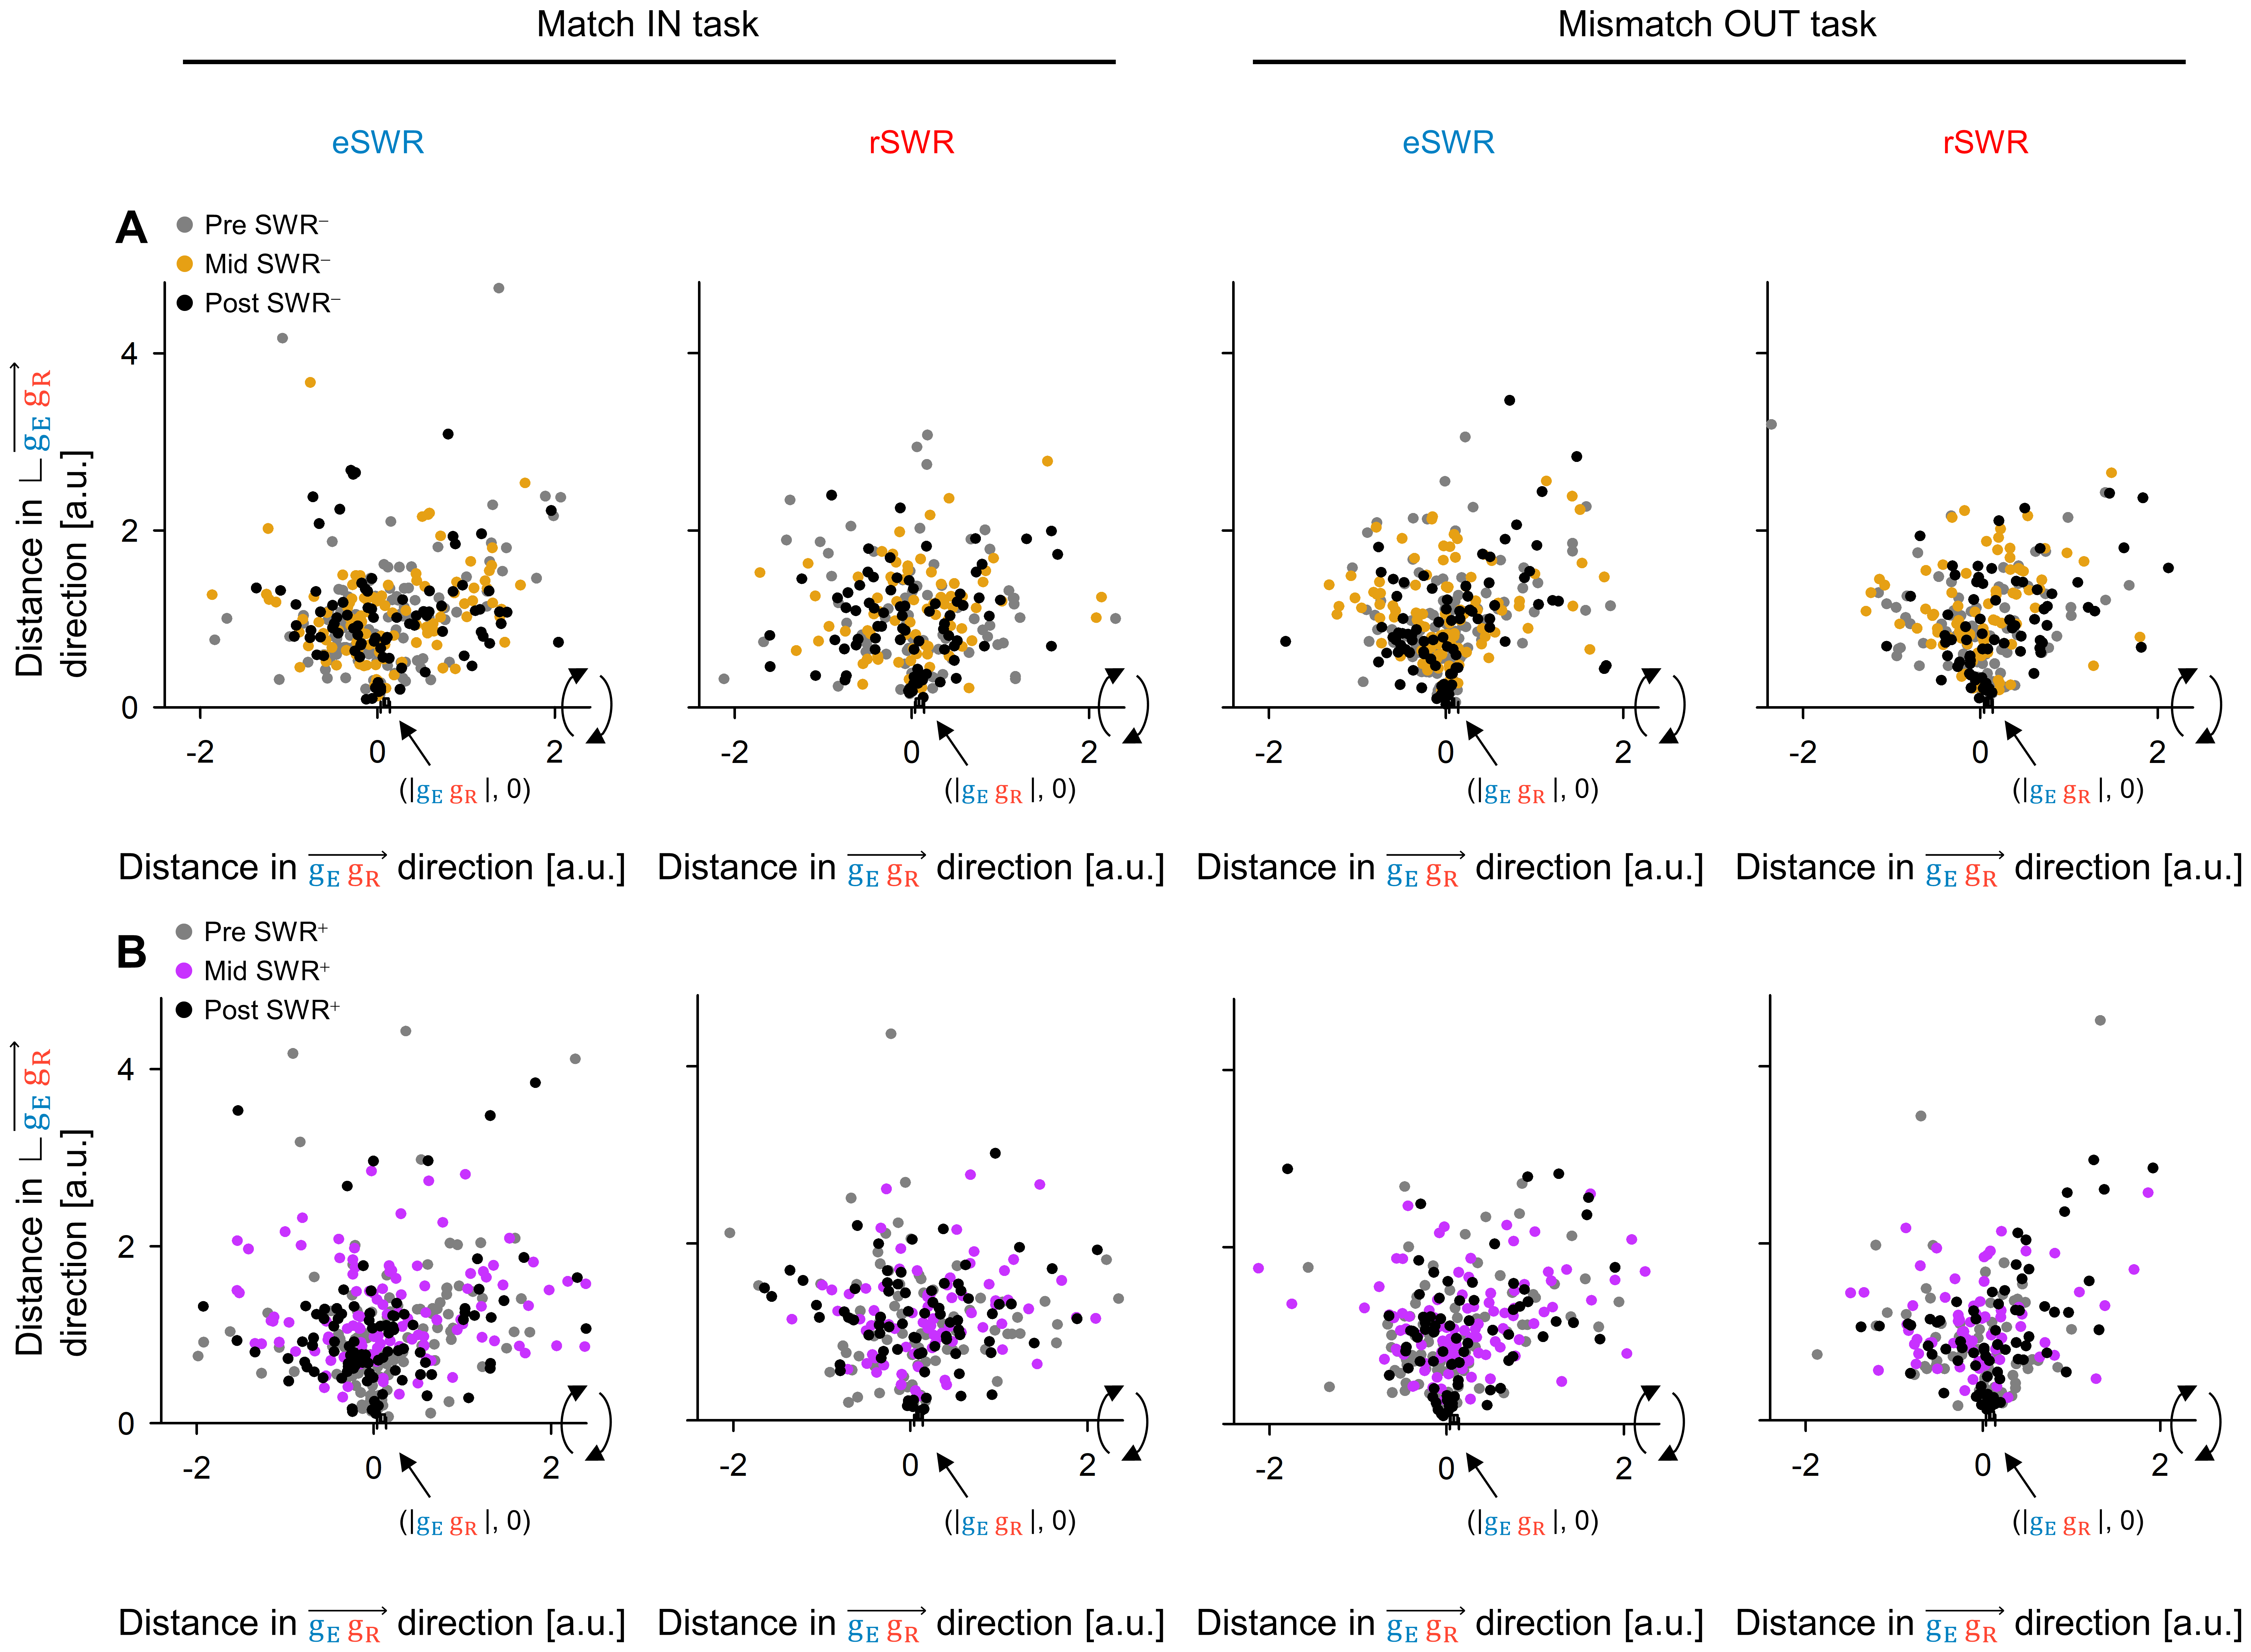
\includegraphics[width=1\textwidth]{./src/figures/.png/Figure_ID_06.png}
%DIFDELCMD <         	%%%
%DIFDELCMD < \caption{%
{%DIFAUXCMD
\textbf{\DIFdelFL{Visualization of Neural Trajectory During SWR in Two-Dimensional Space
}}
%DIFAUXCMD
%DIFDELCMD < \smallskip
%DIFDELCMD < \\
%DIFDELCMD < %%%
\DIFdelFL{The panels depict hippocampal neural trajectories (NTs) during SWR projected onto two-dimensional spaces. }\textbf{\textit{\DIFdelFL{A.}}%DIFAUXCMD
} %DIFAUXCMD
\DIFdelFL{Shows the hippocampal NTs as point clouds during pre-SWR$^-$ (}\textit{\DIFdelFL{gray}}%DIFAUXCMD
\DIFdelFL{), mid-SWR$^-$ (}\textit{\DIFdelFL{yellow}}%DIFAUXCMD
\DIFdelFL{), and post-SWR$^-$ (}\textit{\DIFdelFL{black}}%DIFAUXCMD
\DIFdelFL{). }\textbf{\textit{\DIFdelFL{B.}}%DIFAUXCMD
} %DIFAUXCMD
\DIFdelFL{Conveys the equivalent for SWR$^+$ rather than SWR$^-$. The projection was executed as follows: First, a linear transformation placed $\mathrm{g_{E}}$ at the origin $O$ (0,0), and $\mathrm{g_{R}}$ at ($\lVert \mathrm{g_{E}g_{R}} \rVert$, 0). The point cloud was subsequently rotated around the $\mathrm{g_{E}g_{R}}$ axis (similar to the x axis) for adaptation to two-dimensional spaces. Thus, within these two-dimensional spaces, the distances from point $O$ and the angles for the $\mathrm{g_{E}g_{R}}$ axis are retained as in the original three-dimensional spaces created by GPFA. Abbreviations: SWR denotes sharp-wave ripple events; eSWR refers to SWR during the encoding phase; rSWR signals SWR during the retrieval phase; SWR$^+$, characterizes an SWR event; SWR$^-$ signifies control events for SWR$^+$; pre-SWR, mid-SWR, or post-SWR, represent the time intervals from $-800$ to $-250$ ms, from $-250$ to $+250$ ms, or from $+250$ to $+800$ ms from the center of the SWR.
}}
%DIFAUXCMD
%DIF <  width=1\textwidth
        	%DIFDELCMD < \label{fig:06}
%DIFDELCMD <         \end{figure*}
%DIFDELCMD <         \clearpage
%DIFDELCMD <         \begin{figure*}[ht]
%DIFDELCMD <             %%%
\DIFdelendFL \pdfbookmark[2]{ID 07}{figure_id_07}
        	\centering
            \DIFdelbeginFL %DIFDELCMD < \includegraphics[width=0.5\textwidth]{./src/figures/.png/Figure_ID_07.png}
%DIFDELCMD <         	%%%
\DIFdelendFL \DIFaddbeginFL \includegraphics[width=0.5\textwidth]{./src/figures/png/Figure_ID_07.png}
        	\DIFaddendFL \caption{\textbf{
Direction of Neural Trajectory During SWR Based on Encoding and Retrieval States
}
\smallskip
\\
\textbf{\textit{A--B}} The kernel density estimation distributions of $\protect\overrightarrow{{\mathrm{eSWR^+}}}$ $\cdot$ $\protect\overrightarrow{{\mathrm{rSWR^+}}}$ (\textit{pink circles}), $\protect\overrightarrow{{\mathrm{eSWR^+}}}$ $\cdot$ $\protect\overrightarrow{{\mathrm{g_{E}g_{R}}}}$ (\textit{blue triangles}), and $\protect\overrightarrow{{\mathrm{rSWR^+}}}$ $\cdot$ $\protect\overrightarrow{{\mathrm{g_{E}g_{R}}}}$ (\textit{red rectangles}) in Match In (\textit{A}) and Mismatch OUT tasks (\textit{B}). \textbf{\textit{C--D}} The corresponding distributions of $\mathrm{SWR^-}$ instead of those of $\mathrm{SWR^+}$ in \textit{A} and \textit{B}. \textbf{\textit{E--F}} The differences in the distributions of $\mathrm{SWR^+}$ and those of $\mathrm{SWR^-}$, showing SWR components (\textit{E} = \textit{C} - \textit{A} \& \textit{F} = \textit{D} - \textit{B}). Biphasic distributions of $\protect\overrightarrow{{\mathrm{rSWR^-}}}$ $\cdot$ $\protect\overrightarrow{{\mathrm{g_{E}g_{R}}}}$ indicate fluctuations between the encoding and retrieval states during the Sternberg task. Also, contradicting directionality between $\protect\overrightarrow{{\mathrm{eSWR^+}}}$ and $\protect\overrightarrow{{\mathrm{rSWR^+}}}$ was observed (pink circles) not in Match IN task (\textbf{\textit{E}}), but in Mismatch OUT task (\textbf{\textit{F}}). Lastly, transitions from the retrieval to encoding states are evident in the SWR components in both Match IN and Mismatch OUT tasks (\textit{red rectangles} in \textit{E--F}).
}
% width=0.5\textwidth
        	\label{fig:07}
        \end{figure*}

%%%%%%%%%%%%%%%%%%%%%%%%%%%%%%%%%%%%%%%%%%%%%%%%%%%%%%%%%%%%%%%%%%%%%%%%%%%%%%%%
%% END
%%%%%%%%%%%%%%%%%%%%%%%%%%%%%%%%%%%%%%%%%%%%%%%%%%%%%%%%%%%%%%%%%%%%%%%%%%%%%%%%

\end{document}
